% Required for PDF/A metadata.
% Since LaTeX 2025-11-01, \DocumentMetadata always loads the
% latex-lab tagging modules. This template only needs PDF management
% for the PDF/A metadata, not the experimental tagging layer, so use
% the dedicated pdfmanagement package when it is available.
\IfFileExists{pdfmanagement.sty}{%
  \RequirePackage{pdfmanagement}%
  \SetKeys[document/metadata]{pdfstandard = a-2b, pdfversion = 1.7, lang = sl}%
}{%
  % Compatibility fallback for older TeX installations.
  \providecommand\DebugTemplatesOn{}%
  \providecommand\DebugTemplatesOff{}%
  \DocumentMetadata{pdfstandard = a-2b, pdfversion = 1.7, lang = sl}%
}

% if row numbering is required by your supervisor for review, use the lineno option
\documentclass[9pt]{style/friteza}
% use the following file to define/include additional elements
\graphicspath{{fig/}}

% ------------ additional commands/macros/includes defined by the user
\etal{in sod.}
\renewcommand{\Authands}{ in }
\renewcommand{\Authand}{ in }

\newcommand{\set}[1]{\ensuremath{\mathbf{#1}}}
\renewcommand{\vec}[1]{\ensuremath{\mathbf{#1}}}
\newcommand{\uvec}[1]{\ensuremath{\hat{\vec{#1}}}}
\newcommand{\const}[1]{{\ensuremath{\kappa_\mathrm{#1}}}}

\usepackage{subcaption}
\usepackage{multirow}
\usepackage{tabularx}
\usepackage{csquotes}
\usepackage{svg}
\usepackage{silence}

\usetikzlibrary{arrows.meta, positioning, fit, backgrounds, calc}
\WarningFilter{latex}{Command \showhyphens has changed}

\newmintinline[ltx]{latex}{breaklines}
% --------------------------------------------------
\newcommand{\LeowAWPatchTST}{0{,}64}
\newcommand{\LeowAWPatchTSTRet}{$14{,}6\,\%$}
\newcommand{\LeowAWHistoricalPatchTST}{1{,}42}
\newcommand{\LeowAWHistoricalPatchTSTRet}{$29{,}6\,\%$}
\newcommand{\LeowAWWindowPatchTST}{45}
\newcommand{\LeowAWMarginPatchTST}{-0{,}77}
\newcommand{\LeowAWTFT}{1{,}29}
\newcommand{\LeowAWTFTRet}{$28{,}6\,\%$}
\newcommand{\LeowAWHistoricalTFT}{0{,}46}
\newcommand{\LeowAWHistoricalTFTRet}{$11{,}2\,\%$}
\newcommand{\LeowAWWindowTFT}{64}
\newcommand{\LeowAWMarginTFT}{+0{,}83}
\newcommand{\LeowAWTrainTotal}{38{,}5\,min}
\newcommand{\LeowAWDecisions}{13}
\newcommand{\LeowAWSolvePSO}{67\,ms}
\newcommand{\LeowAWSolveSA}{17\,ms}
\newcommand{\LeowAWTrainPerPatchTST}{17{,}0\,s}
\newcommand{\LeowAWTrainNPatchTST}{65}
\newcommand{\LeowAWTrainPerTFT}{18{,}6\,s}
\newcommand{\LeowAWTrainNTFT}{65}

\newcommand{\WangMASTEROpt}{RD}
\newcommand{\WangMASTER}{1{,}12}
\newcommand{\WangMASTERRet}{$29{,}6\,\%$}
\newcommand{\WangMASTERRisk}{$23{,}1\,\%$}
\newcommand{\WangHistoricalMASTER}{0{,}86}
\newcommand{\WangHistoricalMASTERRet}{$22{,}3\,\%$}
\newcommand{\WangWindowMASTER}{67}
\newcommand{\WangMarginMASTER}{+0{,}26}
\newcommand{\WangTFTOpt}{RD}
\newcommand{\WangTFT}{1{,}79}
\newcommand{\WangTFTRet}{$40{,}2\,\%$}
\newcommand{\WangTFTRisk}{$24{,}6\,\%$}
\newcommand{\WangHistoricalTFT}{1{,}08}
\newcommand{\WangHistoricalTFTRet}{$27{,}8\,\%$}
\newcommand{\WangWindowTFT}{271}
\newcommand{\WangMarginTFT}{+0{,}71}
\newcommand{\WangPatchTSTOpt}{SO}
\newcommand{\WangPatchTST}{1{,}72}
\newcommand{\WangPatchTSTRet}{$37{,}3\,\%$}
\newcommand{\WangPatchTSTRisk}{$22{,}7\,\%$}
\newcommand{\WangHistoricalPatchTST}{1{,}42}
\newcommand{\WangHistoricalPatchTSTRet}{$35{,}7\,\%$}
\newcommand{\WangWindowPatchTST}{336}
\newcommand{\WangMarginPatchTST}{+0{,}30}
\newcommand{\WangSharpeStdMax}{1{,}39}
\newcommand{\WangSharpeStdMin}{0{,}58}
\newcommand{\WangTrainTotal}{$1{,}64$\,h}
\newcommand{\WangSolvePSO}{$2{,}0$\,s}
\newcommand{\WangSolveSA}{$1{,}6$\,s}
\newcommand{\WangTrainPerMASTER}{$33{,}7$\,min}
\newcommand{\WangTrainNMASTER}{1}
\newcommand{\WangTrainPerPatchTST}{$1{,}8$\,min}
\newcommand{\WangTrainNPatchTST}{1}
\newcommand{\WangTrainPerTFT}{$1{,}04$\,h}
\newcommand{\WangTrainNTFT}{1}


%% Enotna višina grafov in ilustracij. Široki shematski sliki
%% (pipeline, protocol_schema) sta izvzeti, ker bi pri tej višini
%% presegli širino stavka.
\newlength{\figheight}
\setlength{\figheight}{150pt}

% Vsak razdelek se začne na svoji strani. titlesec vstavi \sectionbreak pred
% vsak naslov razdelka; \clearpage pred tem izprazni tudi čakajoče plavajoče
% objekte, da ti ne zaidejo v naslednji razdelek.
% (prelom strani samo pred izbranimi razdelki)

\title[slovene]{Optimizacija naložbenih portfeljev z uporabo transformerjev in globalnih optimizacijskih algoritmov}
\title[english]{Investment Portfolio Optimization Using Transformers and Global Optimization Algorithms}

\author{Nejc Škrbec}
% Please give the surname of the lead author for the running footer
\leadauthor{Škrbec N.}

\supervisor{doc. dr.}{Luka Fürst}
% If you do not have a cosupervisor, comment out the following row.
%\cosupervisor{prof. dr.}{Ime Priimek}

% Choose your study programmes (and track, if applicable): BUN-RI, BVS-RI, BUN-RM, BMA-RI-PV, BMA-RI, BMA-MM, BMA-UI
\program{BMA-RI}
% Study-year
\vol{2025/26}
% Choose main language: slovene or english
\mainlanguage{slovene}

\keywords[slovene]{Optimizacija portfelja, Kardinalna omejitev, Transformerji, Napovedovanje donosov, Metahevristike, Rojenje delcev}

\keywords[english]{Portfolio optimization, Cardinality constraint, Transformers, Return forecasting, Metaheuristics, Particle swarm optimization}

% Provide a link (or links) to the repository where your data and code is published. If no code was produced, comment out this section.
\repository{https://github.com/nejcskrbec/portfolio-optimization-using-transformers-and-global-optimization-algorithms}

\sloabstract{V magistrskem delu obravnavamo kardinalno omejeno optimizacijo naložbenih portfeljev, pri kateri sta ključna izziva ocenjevanje pričakovanih donosov in iskanje optimalnih uteži ob zahtevi, da portfelj vsebuje natanko $K$ pozicij. Pričakovane donose ocenjujemo s tremi arhitekturno različnimi transformerskimi modeli (MASTER, TFT in PatchTST), katerih nevronska jedra povzamemo po uradnih izvedbah avtorjev. Kovariančno matriko pri vseh pristopih ocenimo enako iz zgodovinskih donosov, zato primerjava izolira vpliv napovednega signala. Uteži nato optimiziramo z rojenjem delcev in simuliranim ohlajanjem. Oba dela našega optimizacijskega pristopa najprej ovrednotimo ločeno, nato pa skupaj postopno vrednotimo na tes treh objavljenih študij in na lastnem scenariju dolgoročnega vlaganja. V vseh petih preizkusih vsaj en transformerski model preseže svojo ujemajočo zgodovinsko osnovo. PatchTST je najuspešnejši v dolgoročnem scenariju in na naboru DJIA, MASTER na naboru NASDAQ~100, TFT pa v kriznem obdobju.}

\engabstract{This thesis studies cardinality-constrained portfolio optimization, where the two central challenges are estimating expected returns and finding optimal weights subject to the requirement that the portfolio holds exactly $K$ active positions. Expected returns are estimated with three architecturally distinct transformer models (MASTER, TFT and PatchTST), whose neural cores follow the authors' official implementations; our own modifications are restricted to the data interface and to converting the model output into an expected-return estimate. The covariance matrix is estimated identically from historical returns for all approaches, so the comparison isolates the effect of the forecasting signal. Portfolio weights are then optimized with particle swarm optimization and simulated annealing. The forecasting and optimization stages are first evaluated separately, the former with cross-sectional forecasting measures and the latter on the standard OR-Library instances. The complete pipeline is then tested out of sample with walk-forward evaluation on the protocols of three published studies and in an additional long-term investor scenario. In all five experiments at least one transformer clearly beats its matched historical baseline, but which model does so changes systematically with the asset universe and the protocol: PatchTST is strongest in the long-term scenario (Sharpe ratio $1{,}38$ against $1{,}10$ for its baseline) and on DJIA, MASTER on NASDAQ~100 ($1{,}23$ against $1{,}03$), and TFT in the crisis period. Differences between the two optimizers are small and inconsistent, indicating that the quality of the expected-return estimate is the dominant driver of portfolio performance.}

\begin{document}
\maketitle

\dropcap{O}ptimizacija naložbenih portfeljev (v nadaljevanju ONP) predstavlja enega temeljnih problemov kvantitativnih financ. Cilj njenega reševanja je razporediti razpoložljivi kapital med več finančnih sredstev tako, da dosežemo čim ugodnejše razmerje med pričakovanim donosom in tveganjem.

Denimo, da imamo nabor $N$ finančnih sredstev, ki jih spremljamo v diskretnih časovnih korakih $t=0,1,\dots,T$. Ob koncu vsakega trgovalnega dne ima vsako sredstvo določeno zaključno ceno $p_{i,t}$. Enostavni donos $r_{i,t}$ in logaritemski donos $\tilde r_{i,t}$ definiramo z enačbama~\eqref{eq:returns}. Enostavni donos izraža relativno spremembo vrednosti sredstva, logaritemski pa je priročnejši pri modeliranju.

\begin{equation}
\label{eq:returns}
r_{i,t}
=
\frac{p_{i,t}-p_{i,t-1}}{p_{i,t-1}}
=
\frac{p_{i,t}}{p_{i,t-1}}-1,
\qquad
\tilde r_{i,t}
=
\ln\left(
\frac{p_{i,t}}{p_{i,t-1}}
\right).
\end{equation}

V nadaljevanju napovedni horizont označujemo s $H$, ki predstavlja število prihodnjih trgovalnih dni, za katere napovedni model tvori napoved. Glede na uporabljeni model se lahko razlikujeta definicija ciljne spremenljivke in način, kako dnevne napovedi združimo v skupno oceno za izbrani horizont. Konkretno oblikovanje napovedi zato opišemo pri posameznih modelih v razdelku~\ref{sec:mu}.

Donose vseh sredstev v času $t$ zberemo v vektor $\vec{r}_t=(r_{1,t},\dots,r_{N,t})^{\top}$. Portfelj opišemo z vektorjem uteži $\vec{w}=(w_1,\dots,w_N)^{\top}$, kjer $w_i$ predstavlja delež kapitala, vloženega v sredstvo $i$. Donos portfelja $r_t^{\mathrm p}$ opišemo z enačbo~\eqref{eq:portret}.

\begin{equation}
\label{eq:portret}
r_t^{\mathrm p}
=
\vec{w}^{\top}\vec{r}_t.
\end{equation}

Klasično izhodišče za reševanje ONP predstavlja Markowitzev model~\cite{markowitz1952}, ki portfelj obravnava na podlagi pričakovanih donosov sredstev ter njihovega tveganja in medsebojne povezanosti. Prvo opišemo z vektorjem $\vec{\mu}$, tveganje pa s kovariančno matriko $\vec{\Sigma}$. Enačbi obeh zapišemo kot~\eqref{eq:moments}.

\begin{equation}
\label{eq:moments}
\vec{\mu}
=
\mathbb{E}[\vec{r}],
\qquad
\vec{\Sigma}
=
\mathbb{E}
\left[
(\vec{r}-\vec{\mu})
(\vec{r}-\vec{\mu})^{\top}
\right].
\end{equation}

V praksi točnih prihodnjih vrednosti $\vec{\mu}$ in $\vec{\Sigma}$ ne moremo poznati preden se lotimo optimizacije, zato moramo najprej poiskati in kasneje pri optimizaciji uporabiti njuni oceni $\hat{\vec{\mu}}$ in $\hat{\vec{\Sigma}}$. Pri tem je treba upoštevati, da lahko nenatančne ocene pričakovanih donosov vodijo do neugodnega končnega razmerja med donosom in tveganjem v portfelju, tudi kadar je sam optimizacijski postopek izveden optimalno. V razdelku~\ref{sec:mu} podrobneje predstavimo načine ocenjevanja obeh količin, pri čemer se osredotočimo predvsem na uporabo transformerskih modelov za ocenjevanje pričakovanih donosov.

V tej nalogi klasično ONP razširimo z omejitvami, ki bolje odražajo praktične zahteve pri sestavi portfelja. Najpomembnejša je kardinalna omejitev, ki zahteva, da portfelj vsebuje natanko $K$ različnih sredstev. Tako lahko na primer pri oblikovanju portfelja iz univerzuma indeksa S\&P~500 omejimo število izbranih sredstev na vnaprej določeno vrednost $K$. Izbira optimalne vrednosti $K$ predstavlja ločen problem, ki ga v tem delu ne obravnavamo. Za vsako izbrano sredstvo dodatno določimo še najmanjši in največji dovoljeni delež v portfelju. Tako dobimo kardinalno omejeno optimizacijo naložbenega portfelja (v nadaljevanju KONP).

KONP je zahtevnejša od osnovne ONP, ker poleg določanja uteži vključuje tudi diskretno izbiro sredstev: optimizator mora hkrati določiti, katerih $K$ sredstev izmed $N$ bo vključil in kako bo mednje razporedil kapital. Že sam izbor omogoča $\binom{N}{K}$ kombinacij, zato izčrpno iskanje pri večjih problemih hitro postane nepraktično~\cite{chang2000}. V razdelku~\ref{sec:solvers} zato predstavimo dva stohastična globalna optimizacijska algoritma, ki ju uporabimo za reševanje tega problema.

KONP zapišemo z enačbo~\eqref{eq:problem}, ki združuje ocenjeni pričakovani donos portfelja $\hat{\vec{\mu}}^{\top}\vec{w}$ in njegovo ocenjeno tveganje, izraženo s kovariančno matriko $\vec{w}^{\top}\hat{\vec{\Sigma}}\vec{w}$. Parameter $P\in[0,1]$ določa razmerje med njima: večja vrednost daje večjo težo pričakovanemu donosu, manjša pa zmanjševanju tveganja.

Poleg osnovne enačbe moramo nabor veljavnih rešitev KONP omejiti še z nekaj omejitvami. Proračunska omejitev~\eqref{eq:budget} zahteva, da je vsota vseh uteži enaka ena, zato je ves razpoložljivi kapital razporejen med sredstva. Kardinalna omejitev~\eqref{eq:cardinality} zahteva, da je v portfelj vključenih natanko $K$ sredstev, pri čemer binarna spremenljivka $z_i$ določa, ali je sredstvo $i$ vključeno v portfelj. Utežna omejitev~\eqref{eq:c-box} povezuje izbiro sredstva z njegovo utežjo: pri $z_i=0$ mora biti $w_i=0$, pri $z_i=1$ pa mora utež ležati med spodnjo mejo $\varepsilon_i$, ki preprečuje zanemarljivo majhne pozicije, in zgornjo mejo $\delta_i$, ki omejuje koncentracijo kapitala v posameznem sredstvu.

\begin{align}
\max_{\vec{w},\vec{z}}
\quad &
P\,\hat{\vec{\mu}}^{\top}\vec{w}
-
(1-P)\,
\vec{w}^{\top}\hat{\vec{\Sigma}}\vec{w}
\label{eq:problem}
\\
\text{p.p.}\quad
&
\sum_{i=1}^{N} w_i = 1,
\label{eq:budget}
\\
&
\sum_{i=1}^{N} z_i = K,
\label{eq:cardinality}
\\
&
\varepsilon_i z_i
\leq
w_i
\leq
\delta_i z_i,
\qquad
z_i\in\{0,1\},
\quad i=1,\dots,N.
\label{eq:c-box}
\end{align}

V našem delu za reševanje KONP vpeljemo dvostopenjski optimizacijski postopek:

\begin{enumerate}
    \item Najprej ocenimo pričakovane donose $\hat{\vec{\mu}}$. Namesto zgolj zgodovinskega povprečja uporabimo tri arhitekturno različne transformerske modele: PatchTST~\cite{nie2023patchtst}, Temporal Fusion Transformer (TFT)~\cite{lim2021tft} in MASTER~\cite{li2024master}. Njihovo delovanje in način vrednotenja predstavimo v razdelku~\ref{sec:mu}. Pred reševanjem KONP napovedne ocene in oceno tveganja postavimo na skupno skalo, podrobnosti tega postopka pa opišemo v razdelku~\ref{sec:mu}. Kovariančno matriko $\hat{\vec{\Sigma}}$ enostavno ocenimo iz zgodovinskih donosov.

    \item Tako dobljene ocene pričakovanih donosov uporabimo pri reševanju KONP z dvema stohastičnima globalnima optimizacijskima algoritmoma: rojenjem delcev (RD) in simuliranim ohlajanjem (SO). Oba algoritma omogočata iskanje kakovostnih rešitev brez izčrpnega pregleda vseh kombinacij sredstev, vendar prostor rešitev raziskujeta na različna načina. Algoritma podrobneje predstavimo v razdelku~\ref{sec:solvers}.
\end{enumerate}

Eksperimentalna evalvacija postopka poteka v dveh delih. Najprej napovedni in optimizacijski del ovrednotimo ločeno. Napovedne modele ocenimo z merami povezanosti med napovedanimi in realiziranimi donosi, algoritma RD in SO pa na standardnih testnih problemih z znanimi referenčnimi rezultati. Metodologijo vrednotenja in uporabljene mere podrobneje opišemo v razdelku~\ref{sec:impl}.

Nato ovrednotimo še celoten postopek s postopnim vrednotenjem zunaj učnega vzorca (angl.\ \emph{out-of-sample walk-forward evaluation}) na eksperimentalnih scenarijih treh predhodnih raziskav~\cite{leow2021,wang2023oneshot,aprea2026}, ki se razlikujejo po naboru sredstev, časovnem obdobju, pogostosti uravnoteževanja in napovednem obdobju, ter v dodatnem scenariju dolgoročnega vlaganja, v katerem preverimo praktično uporabnost našega pristopa. Rezultate eksperimentalne evalvacije predstavimo v razdelku~\ref{sec:rezultati}, kjer ločeno obravnavamo napovedne in optimizacijske rezultate ter rezultate celotnega postopka.

Osrednji prispevek dela je povezava sodobnih transformerskih napovednih modelov z metahevrističnim reševanjem KONP ter ločeno vrednotenje obeh delov našega pristopa. Tako lahko analiziramo dve povezani vprašanji: ali kakovostnejše napovedi pričakovanih donosov vodijo do uspešnejših portfeljev in koliko je končni rezultat odvisen od uporabljenega optimizacijskega postopka. V sklepu v razdelku~\ref{sec:sklep} povzamemo glavne ugotovitve, omejitve in možnosti za nadaljnje raziskovanje.

\newpage
\section{Sorodna dela}\label{sec:sorodna}

Znanstvene članke, ki si delijo raziskovalno področje z našim delom, lahko razdelimo na tri skupine: optimizacijo portfeljev, napovedovanje prihodnjih donosov in ocenjevanje tveganja. Na vseh treh se je razvoj postopoma premikal od preprostejših statističnih pristopov k metodam, ki lahko obravnavajo več podatkov, več omejitev in zahtevnejše povezave med sredstvi.

\subsection{Optimizacija naložbenih portfeljev}

Po Markowitzevem modelu~\cite{markowitz1952} se je velik del raziskav osredotočil na vprašanje, kako zanesljivi so optimizirani portfelji, kadar so njihovi vhodni podatki ocenjeni iz omejenega nabora. Michaud~\cite{michaud1989} je opozoril, da lahko že majhne napake v ocenjenih donosih povzročijo velike spremembe v sestavi portfelja. Zato so se razvili pristopi, ki skušajo zmanjšati vpliv teh napak. Med najbolj znanimi je Black--Littermanov model~\cite{black1992,helitterman1999}, ki pri oblikovanju ocen prihodnjih donosov upošteva dodatne informacije o trgu. Empirične primerjave so hkrati pokazale, da zahtevnejša optimizacija ni vedno uspešnejša od preprostih strategij~\cite{demiguel2009,bessler2017,tu2011}.

Omenimo še pristope k reševanju KONP\@. Zgodnejše raziskave so uporabljale natančne matematične postopke~\cite{bienstock1996,gao2013}, vzporedno pa so se razvijali tudi hevristični pristopi, ki iščejo kakovostne rešitve brez preiskovanja vseh možnih kombinacij~\cite{chang2000}. Kasnejše metode so problem poskušale poenostaviti tako, da spodbujajo manjše število izbranih sredstev~\cite{brodie2009,kim2016sparse}, ali pa so združile več različnih načinov iskanja in določanja uteži~\cite{akbay2020}.

\subsection{Napovedovanje pričakovanih donosov}

Zgodnejše raziskave napovedovanja donosov so iskale predvsem ponavljajoče se zakonitosti v preteklih podatkih in ekonomskih značilnostih sredstev. Primer je moment, pri katerem imajo sredstva z relativno boljšimi preteklimi donosi v določenih obdobjih težnjo, da ostanejo uspešnejša tudi v bližnji prihodnosti~\cite{jegadeesh1993,carhart1997}. Takšni pristopi temeljijo predvsem na vnaprej določenih signalih. Z večjo količino razpoložljivih podatkov pa so se začele uporabljati metode strojnega učenja, ki lahko same poiščejo uporabne nelinearne povezave med večjim številom značilk~\cite{gu2020}. Med takšne pristope sodijo tudi modeli, kot je LightGBM~\cite{ke2017lightgbm}.

Naslednji korak je bil neposredno modeliranje časovnega razvoja podatkov z nevronskimi mrežami. Selvin in sod.~\cite{selvin2017stock} so pri napovedovanju cen delnic primerjali več rekurentnih in konvolucijskih arhitektur. Modeli, kot je LSTM~\cite{hochreiter1997lstm}, so bili pri tem zanimivi predvsem zato, ker lahko pri napovedi upoštevajo informacije iz daljšega zaporedja preteklih opazovanj. Napovedni modeli so se začeli vključevati tudi neposredno v postopke sestave portfeljev. Barua in Sharma~\cite{barua2022} sta na primer napovedi nevronskega modela uporabila kot vhod v Black--Littermanov pristop.

Novejši razvoj predstavljajo arhitekture s pozornostjo in transformerji~\cite{vaswani2017}. Ti omogočajo, da model pri napovedi neposredno ovrednoti pomen različnih delov vhodnega zaporedja, zato so postali zanimivi tudi za finančne časovne vrste~\cite{wang2022,zhang2022transformer}. Vzporedno so se razvili splošnejši modeli za napovedovanje časovnih vrst~\cite{wu2021autoformer,das2024timesfm}. Raziskave se hkrati vse bolj oddaljujejo od obravnave posamezne delnice kot izoliranega zaporedja. Nekateri modeli upoštevajo povezave med različnimi delnicami~\cite{ye2020multigraph,li2020graphstock}, drugi pa cenovne podatke dopolnjujejo z novicami, besedili in informacijami o podjetjih~\cite{sawhney2020deep,cheng2022multimodality}. Leow in sod.~\cite{leow2021} so na primer razpoloženje iz družbenih omrežij, ki ga zajamejo z modelom BERT, prek genetskega algoritma vključili v klasično sestavo portfelja; njihovo delo uporabimo kot zunanjo referenčno primerjavo v razdelku~\ref{sec:leow}. V našem delu iz tega širšega razvoja izberemo TFT~\cite{lim2021tft}, MASTER~\cite{li2024master} in PatchTST~\cite{nie2023patchtst}, ki predstavljajo tri različne načine uporabe transformerjev za napovedovanje časovnih vrst in finančnih donosov.

\subsection{Ocenjevanje tveganja in kovariančne matrike}

Pri sestavi portfelja moramo poleg prihodnjih donosov oceniti tudi tveganje in povezanost med sredstvi. Osnovna težava je, da pri večjem številu sredstev hitro naraste število povezav, ki jih moramo oceniti iz omejenega števila opazovanj. Raziskave so zato iskale načine, kako ocenjevanje poenostaviti ali stabilizirati. Faktorski modeli skupno gibanje velikega števila sredstev opišejo z manjšim številom skupnih dejavnikov~\cite{fan2008}. Druga smer upošteva, da se tveganje in povezanost med sredstvi skozi čas spreminjata, zato ju modelira dinamično~\cite{engle2002,chiriac2011}.

Pomemben pristop je tudi neposredna stabilizacija kovariančne matrike, saj je vzorčna cenilka pri omejenem številu opazovanj lahko zelo nestabilna. Novejše raziskave to težavo rešujejo z metodami strojnega učenja. Nekateri pristopi se iz podatkov učijo skupnih dejavnikov tveganja~\cite{lin2021deeprisk}, drugi pa poskušajo izboljšati samo oceno kovariančne matrike~\cite{yang2025}. Še druga možnost je, da namesto posameznih kovarianc modeliramo skupno porazdelitev več časovnih vrst; tak primer je GPVar~\cite{salinas2019}. V tej nalogi se osredotočimo predvsem na vpliv napovedi pričakovanih donosov, zato pri vseh treh transformerskih modelih uporabimo isto vzorčno kovariančno matriko zgodovinskih donosov. S tem pri primerjavi napovednih modelov ohranimo nespremenjen vhod, ki opisuje tveganje.

%% ============================================================
% FORECASTING
% ============================================================

\section{Napovedovanje pričakovanih donosov}\label{sec:mu}

V našem delu $\hat{\vec{\mu}}$ pridobimo s tremi transformerskimi modeli: PatchTST~\cite{nie2023patchtst}, Temporal Fusion Transformer (TFT)~\cite{lim2021tft} in MASTER~\cite{li2024master}. Postopek učenja je skupen vsem trem napovednim modelom in je opisan v razdelku~\ref{sec:forecast-pipeline}.

% ------------------------------------------------------------
% PatchTST
% ------------------------------------------------------------

\subsection{PatchTST}\label{sec:patchtst}~\cite{nie2023patchtst} je transformerski model za napovedovanje večspremenljivih časovnih vrst. Večspremenljiva časovna vrsta vsebuje več spremenljivk, opazovanih skozi čas, medtem ko univariatna časovna vrsta vsebuje le eno spremenljivko. Njegovi ključni značilnosti sta razdelitev vhodnega zaporedja na krajše odseke (angl.\ \emph{patches}) in neodvisna obravnava posameznih kanalov. Kanal predstavlja eno univariatno časovno vrsto. V našem primeru posamezen kanal predstavlja dnevne logaritemske donose enega finančnega sredstva. Če spremljamo $N$ sredstev v $L$ zaporednih dneh, vhod predstavlja matrika velikosti $L\times N$, pri čemer vsak stolpec predstavlja en kanal. PatchTST kanale obravnava ločeno, vendar med njimi deli iste naučene parametre, kar avtorji imenujejo neodvisnost kanalov (angl.\ \emph{channel independence}).

Naj bo $L$ dolžina vhodnega zaporedja, $P$ dolžina posameznega odseka in $S$ korak med začetkoma dveh zaporednih odsekov. Če je $S<P$, se odseki prekrivajo. Večji $L$ omogoča uporabo daljšega zgodovinskega konteksta, večji $P$ pa zajame več lokalnega časovnega konteksta v posameznem žetonu. Razdelitev na odseke zmanjša število vhodnih žetonov, kar zmanjša računsko in pomnilniško zahtevnost modela.

Vsak odsek se z naučljivo linearno preslikavo preslika v notranji prostor dimenzije $D$, nato pa se mu doda pozicijska vdelava, ki ohrani informacijo o njegovem položaju v zaporedju. Zaporedje tako dobljenih žetonov nato obdela transformerski kodirnik, ki s samopozornostjo modelira odvisnosti med različnimi odseki. Končna predstavitev se uporabi za napoved prihodnjih vrednosti.

Osnovne arhitekture modela ne spreminjamo, saj smo jo prevzeli iz uradnega repozitorija avtorjev~\cite{nie2023patchtst_code}. Za reševanje KONP z modelom za posamezno sredstvo napovedujemo dnevne logaritemske donose $\hat{\tilde r}_{i,t+h}$ za naslednjih $H$ dni ($h=1,\dots,H$). Iz njih izračunamo $H$-dnevni enostavni donos po enačbi~\eqref{eq:patchtst-return}, napovedi vseh sredstev pa nato zberemo v vektor $\hat{\vec{\mu}}_{\mathrm{PatchTST}}$.

\begin{equation}
\label{eq:patchtst-return}
r_{i,t}^{(H)}
=
\exp\left(
\sum_{h=1}^{H}\tilde r_{i,t+h}
\right)-1.
\end{equation}

% ------------------------------------------------------------
% TFT
% ------------------------------------------------------------

\subsection{Temporal Fusion Transformer}\label{sec:tft}~\cite{lim2021tft} je transformerski model za večhorizontno napovedovanje časovnih vrst, zasnovan za delo z različnimi vrstami vhodnih značilk. Model podpira tri glavne skupine značilk, ki jih obravnava z mehanizmom izbire spremenljivk (angl.\ \emph{variable selection}), rekurentnimi plastmi LSTM in časovno samopozornostjo (angl.\ \emph{temporal self-attention}). Tri vrste značilk so naslednje:

\begin{enumerate}
    \item \textbf{Statične značilke} (angl.\ \emph{static covariates}) se skozi čas ne spreminjajo (npr.\ kategorija, identifikator). Pri reševanju KONP posamezno sredstvo predstavlja eno časovno vrsto zato kot statično značilko uporabimo oznako sredstva (angl.\ \emph{ticker}). Statične značilke model predstavi z naučljivo vdelavo, s čimer lahko pri skupnem učenju razlikuje med posameznimi časovnimi vrstami.
    \item \textbf{Časovno spremenljive opazovane značilke} (angl.\ \emph{time-varying observed variables}) imajo vrednosti, ki so nam znane do trenutka napovedi, prihodnje vrednosti pa niso znane (npr.\ zgodovinske vrednosti). Pri reševanju KONP sem spadajo dnevni logaritemski donosi $\tilde r_{i,t}$. Poleg njih pa uporabimo še 20-dnevni momentum, ki povzame kumulativno gibanje cene sredstva in pa 20-dnevno volatilnost, ki meri variabilnost dnevnih donosov v zadnjem obdobju. Vse tri časovno spremenljive opazovane značilke v naši implementaciji izračunamo iz zaključnih cen sredstev. 
    \item \textbf{Časovno spremenljive znane značilke} (angl.\ \emph{ti
    me-varying known variables}) so značilnosti, katerih prihodnje vrednosti so ob trenutku napovedi že znane (npr.\ datum, dan v tednu, praznik ali vnaprej določen urnik). Takšnih značilk pri reševanju KONP ne uporabljamo.
\end{enumerate}

TFT implementiramo z modelom \texttt{TemporalFusionTransformer} iz knjižnice \texttt{pytorch-forecasting}~\cite{beitner2020pytorch}. Ciljna spremenljivka je dnevni logaritemski donos $\tilde r_{i,t}$ posameznega sredstva. Model je zasnovan za kvantilno regresijo, pri kateri za vsak prihodnji dan napove več kvantilov ciljnega donosa. Kvantil določa mejo določenega deleža napovedanih vrednosti, pri čemer $q=0{,}5$ predstavlja mediano. V naši implementaciji iz izračunanih kvantilov uporabimo kvantil $q=0{,}5$ in tako dobimo eno napovedano vrednost dnevnega logaritemskega donosa $\hat{\tilde r}_{i,t+h}$ za vsakega od naslednjih $H$ dni ($h=1,\dots,H$). Te dnevne napovedi nato združimo v napoved $H$-dnevnega enostavnega donosa po enačbi~\eqref{eq:patchtst-return}, napovedi vseh $N$ sredstev pa zberemo v vektor $\hat{\vec{\mu}}_{\mathrm{TFT}}$.

% ------------------------------------------------------------
% MASTER
% ------------------------------------------------------------

\subsection{MASTER}\label{sec:master}

MASTER~\cite{li2024master} je transformerski model, namenjen napovedovanju standardizirane vrednosti prihodnjega donosa delnic. Za posamezno sredstvo $u$ in napovedni horizont $H$ je osnova za ciljno spremenljivko prihodnji $H$-dnevni enostavni donos, ki ga definiramo z enačbo~\eqref{eq:master-target}.

\begin{equation}
\label{eq:master-target}
r_{u,t}^{\mathrm{MASTER}}
=
\frac{p_{u,t+H}}{p_{u,t+1}}-1.
\end{equation}

Pri učenju ta donos za vsak datum presečno standardiziramo, kar pomeni, da od posameznega donosa odštejemo povprečje donosov vseh sredstev na istem datumu in rezultat delimo z njihovim standardnim odklonom. MASTER tako napoveduje standardizirano vrednost prihodnjega donosa, ki predstavlja njegov relativni položaj glede na druga sredstva na istem datumu. Poleg časovnih vzorcev znotraj posameznega sredstva modelira tudi presečne povezave med sredstvi. Njegova ključna značilnost je tržno vodeno uteževanje značilk (angl.\ \emph{market-guided gating}), pri katerem tržni kontekst vpliva na uteževanje vhodnih značilk. Model nato informacije obdeluje z agregacijo znotraj sredstva (angl.\ \emph{intra-stock aggregation}), agregacijo med sredstvi (angl.\ \emph{inter-stock aggregation}) in časovno agregacijo (angl.\ \emph{temporal aggregation})~\cite{li2024master}.

Arhitekture modela ne spreminjamo, saj smo jo povzeli iz uradnega repozitorija avtorjev~\cite{li2024master_code}, prilagodili pa smo pripravo vhodnih značilk za uporabo modela na ameriških delnicah. MASTER je bil izvorno razvit in ovrednoten na kitajskih delnicah ter uporablja podatkovno infrastrukturo Qlib~\cite{yang2020qlib}, odprtokodno platformo za kvantitativne raziskave in strojno učenje na finančnih podatkih. Za posamezno sredstvo model prejme 158 značilk Alpha158~\cite{yang2020qlib}, izpeljanih iz dnevnih podatkov OHLCV (cena ob odprtju, najvišja in najnižja cena, cena ob zaprtju ter promet). Značilke Alpha158 smo v naši implementaciji ponovno izračunali iz podatkov OHLCV, prenesenih prek knjižnice \texttt{yfinance}. Vse vhodne značilke robustno normaliziramo na podlagi mediane in mediane absolutnih odklonov (MAD), da zmanjšamo vpliv ekstremnih vrednosti na napovedi modela. Parametre normalizacije ocenimo izključno na učnem obdobju, normalizirane vrednosti omejimo na interval $[-3,3]$, manjkajoče vrednosti pa nadomestimo z nič.

Poleg značilk posameznega sredstva model uporablja tudi skupni tržni vektor $\vec{m}_t$, ki je enak za vsa sredstva. V naši implementaciji ga sestavlja 63 značilk, izpeljanih iz treh ameriških ETF-ov SPY, IWM in VTI ter njihovih dnevnih donosov, kotalnega povprečja in standardnega odklona donosov ter kotalnega povprečja in standardnega odklona zneska trgovanja na oknih 5, 10, 20, 30 in 60 dni.

Za posamezen napovedni dan model uporablja časovno okno osmih trgovalnih dni, zato je vhodni tenzor oblike $[N,8,221]$, kjer je $N$ število sredstev, 221 pa predstavlja 158 značilk posameznega sredstva in 63 skupnih tržnih značilk. Ciljna oznaka je shranjena v 222.\ stolpcu.

Pri uporabi modela za napovedi izhode MASTER zberemo za vsa razpoložljiva sredstva in jih presečno standardiziramo v $z$-vrednosti, tako da od vsake napovedi odštejemo povprečje napovedi vseh sredstev ter rezultat delimo z njihovim standardnim odklonom. Za razliko od PatchTST in TFT MASTER ne napoveduje dnevnih logaritemskih donosov, iz katerih bi nato izračunali večdnevni donos, temveč neposredno vrne en napovedni signal za posamezno sredstvo. Tako dobljene standardizirane vrednosti zberemo v vektor $\hat{\vec{\mu}}_{\mathrm{MASTER}}$, ki ga uporabimo kot napovedni vhod v portfeljski optimizaciji.

% ============================================================
% COVARIANCE
% ============================================================

\subsection{Ocena kovariančne matrike}\label{sec:cov}

Pri primerjavi napovednih modelov želimo spreminjati predvsem vir ocene $\hat{\vec{\mu}}$, zato kovariančno matriko pri vseh pristopih ocenimo na enak način.

Naj bo v trenutnem ocenjevalnem oknu na voljo $T_w$ vektorjev donosov $\vec{r}_t$. Vzorčno povprečje donosov in vzorčno kovariančno matriko definiramo z enačbo~\eqref{eq:sample-moments}:
\begin{equation}
\label{eq:sample-moments}
\begin{aligned}
\bar{\vec{r}}
&=
\frac{1}{T_w}
\sum_{t=1}^{T_w}\vec{r}_t,
\qquad
&
\hat{\vec{\Sigma}}
&=
\frac{1}{T_w-1}
\sum_{t=1}^{T_w}
(\vec{r}_t-\bar{\vec{r}})
(\vec{r}_t-\bar{\vec{r}})^{\top}.
\end{aligned}
\end{equation}

Če je zaradi numerične natančnosti potrebno, matriki $\hat{\vec{\Sigma}}$ dodamo majhen diagonalni popravek. Ker je kovariančna matrika pri zgodovinskem pristopu, TFT, MASTER in PatchTST ocenjena na enak način po enačbi~\eqref{eq:sample-moments}, lahko razlike v končnih portfeljih lažje povežemo z razlikami v ocenah pričakovanih donosov.

Dolžino ocenjevalnega okna $T_w$ izberemo enako najdaljšemu pogojnemu oknu med modeli v posameznem eksperimentu. S tem sta oba vhoda optimizatorja, $\hat{\vec{\mu}}$ in $\hat{\vec{\Sigma}}$, ocenjena na primerljivi nedavni zgodovini: noben model ni v primerjavi s kovarianco, ocenjeno iz bistveno daljšega obdobja, ki ga sam nikoli ne vidi.


% ============================================================
% SOLVERS
% ============================================================

\clearpage
\section{Globalni optimizacijski algoritmi}\label{sec:solvers}

Ker algoritmi KONP rešujejo z minimizacijo, ciljno funkcijo iz enačbe~\eqref{eq:problem} zapišemo v ekvivalentni obliki~\eqref{eq:solver-objective}, kjer manjša vrednost $g(\vec{w})$ pomeni boljšo rešitev.

\begin{equation}
\label{eq:solver-objective}
g(\vec{w})
=
(1-P)\vec{w}^{\top}\hat{\vec{\Sigma}}\vec{w}
-
P\hat{\vec{\mu}}^{\top}\vec{w}.
\end{equation}

Kandidatna rešitev predstavlja portfelj, torej izbor sredstev in njihove uteži, in mora zadovoljiti vse omejitve KONP iz enačb~\eqref{eq:budget}--\eqref{eq:c-box}. Ker naključni premiki teh omejitev ne ohranijo samodejno, rešitve po potrebi popravimo.

% ------------------------------------------------------------
% RD
% ------------------------------------------------------------

\subsection{Rojenje delcev (RD)}\label{sec:rd}
(angl.\ \emph{Particle Swarm Optimization}, PSO)~\cite{kennedy1995} je populacijski optimizacijski algoritem, navdihnjen z vedenjem skupin živali, kot so jate ptic ali rib ter roji žuželk. V našem delu smo uporabili različico RD, prilagojeno za reševanje KONP~\cite{cura2009}.

Denimo, da imamo populacijo delcev, kjer vsak delec predstavlja kandidatno rešitev. Vsak delec pri iskanju rešitve upošteva svojo najboljšo doslej najdeno rešitev in najboljšo rešitev celotne populacije. Nek delec $m$ opišemo z dvojico $(\vec{x}_m,\vec{z}_m)$, kjer $\vec{x}_m$ predstavlja položaj delca oziroma vektor uteži izbranih sredstev, $\vec{z}_m$ pa z binarnimi vrednostmi označuje izbor sredstev. Za obe komponenti delec hrani hitrosti $\vec{v}^{\,x}_m$ in $\vec{v}^{\,z}_m$ ter svojo najboljšo doslej obiskano rešitev $(\vec{x}_m^\star,\vec{z}_m^\star)$. Najboljšo rešitev celotnega roja določimo z delcem z najboljšo osebno rešitvijo.

V vsaki iteraciji za vsak delec $m$ in vsako sredstvo $i$ izvedemo naslednje korake:

\begin{enumerate}
    \item \textbf{Posodobitev izbora sredstev.}
    Neodvisno vzorčimo $\omega_1,\omega_2\sim U[0,2]$. Binarno hitrost določimo z enačbo~\eqref{eq:pso-binary-velocity}, pri čemer prva komponenta usmerja delec proti globalno najboljši rešitvi, druga pa proti njegovi osebno najboljši rešitvi.
    
    \begin{equation}
    \label{eq:pso-binary-velocity}
    v^{z,t+1}_{m,i}
    =
    v^{z,t}_{m,i}
    +
    \omega_1\left(z_i^{G}-z^{t}_{m,i}\right)
    +
    \omega_2\left(z^{\star}_{m,i}-z^{t}_{m,i}\right).
    \end{equation}

    Novo vrednost vsake komponente vektorja izbora sredstev $z_{m,i}$ določimo tako, da vrednost $z^t_{m,i}+v^{z,t+1}_{m,i}$ najprej s sigmoidno funkcijo preslikamo v interval $(0,1)$, nato pa jo glede na prag pretvorimo v binarno vrednost $z^{t+1}_{m,i}\in\{0,1\}$, kot določa enačba~\eqref{eq:pso-binary-position}. $\alpha=0{,}06$ je odmik, ki vpliva na prag izbora sredstva.

    \begin{equation}
    \label{eq:pso-binary-position}
    z^{t+1}_{m,i}
    =
    \left\lfloor
    S\left(z^{t}_{m,i}+v^{z,t+1}_{m,i}\right)-\alpha+\frac{1}{2}
    \right\rfloor,
    \qquad
    S(a)=\frac{1}{1+e^{-a}},
    \end{equation}

    \item \textbf{Posodobitev uteži sredstev.}
    Če je sredstvo po prejšnjem koraku izbrano, hitrost posodobimo z enačbo~\eqref{eq:pso-continuous-velocity}, pri čemer se delec pomika proti globalno in osebno najboljši rešitvi. Nato položaj posodobimo po enačbi~\eqref{eq:pso-continuous-position}. Če je sredstvo ni izbrano, v naši implementaciji njegovo vrednost $x^{t+1}_{m,i}$ nastavimo na nič, hitrost $v^{x,t+1}_{m,i}$ pa ohranimo.
    
    \begin{equation}
    \label{eq:pso-continuous-velocity}
    v^{x,t+1}_{m,i}
    =
    v^{x,t}_{m,i}
    +
    \omega_1\left(x_i^{G}-x^{t}_{m,i}\right)
    +
    \omega_2\left(x^{\star}_{m,i}-x^{t}_{m,i}\right).
    \end{equation}

    \begin{equation}
    \label{eq:pso-continuous-position}
    x^{t+1}_{m,i}
    =
    x^{t}_{m,i}
    +
    v^{x,t+1}_{m,i}.
    \end{equation}

    \item \textbf{Popravljanje kardinalnosti.}
    Posodobitev izbora sama po sebi ne zagotavlja natanko $K$ izbranih sredstev, zato po vsakem premiku izvedemo popravljanje kardinalnosti. Če je izbranih manj kot $K$ sredstev, z enako verjetnostjo dodamo naključno neizbrano sredstvo ali neizbrano sredstvo z največjo vrednostjo $c_i$. Če jih je izbranih več kot $K$, na enak način odstranimo naključno sredstvo ali sredstvo z najmanjšo vrednostjo $c_i$. Avtorji~\cite{cura2009} mero $c_i$ definirajo iz pričakovanega donosa in povprečne kovariance sredstva glede na stopnjo averzije do tveganja. Vmesne količine $\theta_i$ in $\rho_i$ ter korekcijska odmika $\Omega$ in $\Psi$ določimo po enačbi~\eqref{eq:pso-correction}. Ker so $\hat{\vec{\mu}}$, $\hat{\vec{\Sigma}}$ in $\lambda$ v posameznem optimizacijskem oknu nespremenljivi, $c_i$ v naši implementaciji izračunamo le enkrat pred začetkom iteracij.

    \begin{equation}
    \label{eq:pso-correction}
    \begin{aligned}
    \theta_i &= 1+(1-\lambda)\hat{\mu}_i,
    &
    \rho_i &= 1+\lambda\,\frac{1}{N}\sum_{j=1}^{N}\hat{\Sigma}_{ij},
    \\
    c_i &= \frac{\theta_i+\Omega}{\rho_i+\Psi},
    &
    \Omega &= -\min\left(0,\min_j\theta_j\right),
    \qquad
    \Psi = -\min\left(0,\min_j\rho_j\right).
    \end{aligned}
    \end{equation}

    \item \textbf{Projekcija uteži.}
    Po popravilu kardinalnosti uporabimo funkcijo \texttt{normalize\_weights}, ki izbranim sredstvom določi uteži, skladne s proračunsko ter spodnjo in zgornjo utežno omejitvijo.
\end{enumerate}

\begin{algorithm}[H]
\caption{Rojenje delcev za KONP~\cite{cura2009}}
\label{alg:pso}
\begin{algorithmic}[1]
\State \textbf{Vhod:} ocene donosov $\hat{\vec{\mu}}$, kovariančna matrika $\hat{\vec{\Sigma}}$, parameter tveganja $P$, kardinalnost $K$, velikost roja $M$, število iteracij $T$
\State \textbf{Izhod:} najboljše uteži $\textit{best\_weights}$
\State izračunaj $c_i$ za vsa sredstva po~\eqref{eq:pso-correction} \label{ln:pso-score}
\State ustvari $M$ naključnih delcev z natanko $K$ izbranimi sredstvi in dopustnimi utežmi \label{ln:pso-init}
\ForAll{$\textit{particle} \in \textit{swarm}$}
    \State $\textit{particle.fit} \leftarrow f(\textit{particle})$
    \State $\textit{particle.best\_fit} \leftarrow \textit{particle.fit}$
    \State $\textit{particle.best\_weights} \leftarrow \textit{particle.weights}$
    \State $\textit{particle.best\_selection} \leftarrow \textit{particle.selection}$
\EndFor
\State $\textit{leader} \leftarrow$ delec z najmanjšo vrednostjo $\textit{best\_fit}$ \label{ln:pso-leader}
\For{$t=1,\dots,T$}
    \ForAll{$\textit{particle} \in \textit{swarm}$} \label{ln:pso-loop}
        \For{$i=1,\dots,N$}
            \State $\omega_1,\omega_2 \sim U[0,2]$
            \State posodobi $v^{z,t+1}_{m,i}$ po~\eqref{eq:pso-binary-velocity}
            \State posodobi $z^{t+1}_{m,i}$ po~\eqref{eq:pso-binary-position}
            \If{$z^{t+1}_{m,i}=1$}
                \State posodobi $v^{x,t+1}_{m,i}$ po~\eqref{eq:pso-continuous-velocity}
                \State posodobi $x^{t+1}_{m,i}$ po~\eqref{eq:pso-continuous-position}
            \Else
                \State $x^{t+1}_{m,i} \leftarrow 0$
            \EndIf
        \EndFor
        \State popravi izbor tako, da je izbranih natanko $K$ sredstev, z uporabo $c_i$ \label{ln:pso-fix}
        \State projiciraj uteži na dopustno množico
        \State $\textit{particle.fit} \leftarrow f(\textit{particle})$ \label{ln:pso-eval}
        \If{$\textit{particle.fit} < \textit{particle.best\_fit}$}
            \State posodobi osebno najboljšo rešitev delca
        \EndIf
        \If{$\textit{particle.best\_fit} < \textit{leader.best\_fit}$}
            \State $\textit{leader} \leftarrow \textit{particle}$
        \EndIf
    \EndFor
\EndFor
\State $\textit{best\_weights} \leftarrow \textit{leader.best\_weights}$
\State \Return $\textit{best\_weights}$
\end{algorithmic}
\end{algorithm}
Slika~\ref{fig:pso-illus} prikazuje poenostavljeno ponazoritev delovanja roja delcev v dvodimenzionalnem prostoru, kjer posamezna točka predstavlja eno možno rešitev. Izolinije prikazujejo vrednosti ciljne funkcije $f(\vec{w})=-\mathrm{Sharpe}(\vec{w})$, pri čemer nižje vrednosti pomenijo boljše rešitve, minimum pa predstavlja optimalno rešitev $\vec{w}^{\ast}$. V prvi iteraciji je pet delcev (I--V) naključno razporejenih po prostoru, vsak pa svojo začetno pozicijo shrani kot osebno najboljšo rešitev. V drugi iteraciji se delci premaknejo na podlagi svojih hitrosti; na smer in velikost premika vplivata njihova osebno najboljša rešitev ter najboljša rešitev celotnega roja. V iteraciji~$t$ je za delec~II podrobneje prikazano, kako se njegova nova hitrost sestavi iz predhodne hitrosti ter komponent, usmerjenih proti osebno najboljši in globalno najboljši rešitvi. Posodobljena hitrost nato določi nov položaj delca. Z večanjem števila iteracij se roj zaradi skupnega vpliva teh dveh informacij postopoma pomika proti območjem z nižjo vrednostjo ciljne funkcije.

% TODO: Popravi sliko, da bo uporabljala dejansko ciljno funkcijo

\begin{figure}[htbp]
    \centering
    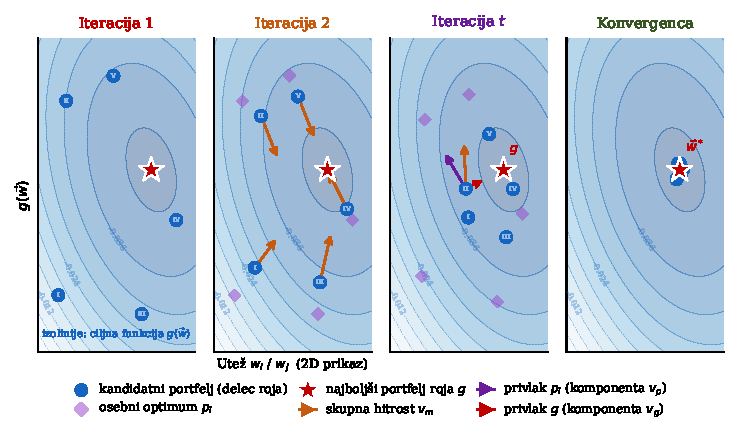
\includegraphics[height=\figheight]{fig/optimizer_pso_illus.pdf}
    \caption{Poenostavljena ponazoritev gibanja roja delcev v dvodimenzionalnem prostoru.}
    \label{fig:pso-illus}
\end{figure}
% ------------------------------------------------------------
% SO
% ------------------------------------------------------------
\newpage
\subsection{Simulirano ohlajanje (SO)}\label{sec:so} (angl.\ \emph{Simulated Annealing})~\cite{kirkpatrick1983} je metahevristični optimizacijski algoritem, ki ima analogijo s procesom ohlajanja materiala. V našem delu smo SO prilagodili za reševanje kardinalno omejenega portfeljskega problema (KONP), pri čemer posamezne mehanizme algoritma povzemamo po literaturi..

Osnovna ideja SO je, da algoritem poleg izboljšav občasno sprejme tudi slabše rešitve, s čimer se izogiba lokalnim minimumom in učinkoviteje raziskuje prostor rešitev. Verjetnost sprejema slabše rešitve je odvisna od temperature $T$: pri višjih temperaturah je večja, z njenim zniževanjem pa postaja algoritem vse bolj selektiven.

Za razliko od RD simulirano ohlajanje ne vzdržuje populacije kandidatov, temveč eno trenutno rešitev $\vec{w}$, katere soseščino zaporedno preiskuje. Ključna sestavina algoritma je temperaturni urnik (angl.\ \emph{cooling schedule}), ki določa način zniževanja temperature skozi iteracije; v naši implementaciji sta osnovna parametra začetna temperatura $T_0$ in geometrijsko ohlajanje s faktorjem $\alpha_{\mathrm{SO}}$.

Iskanje poteka po naslednjih korakih:
\begin{enumerate}
    \item \textbf{Inicializacija portfelja.}
    Algoritem začnemo z naključno izbranimi $K$ sredstvi, vsako dobi utež $1/K$. Začetni portfelj $\vec{w}$ tako že zadovoljuje kardinalno, proračunsko ter spodnjo in zgornjo utežno omejitev..

    \item \textbf{Generiranje sosednje rešitve.}
    Sosednostna funkcija (angl.\ \emph{neighborhood function}) iz trenutne rešitve ustvari eno kandidatno rešitev na enega od dveh načinov:
    \begin{enumerate}
        \item \textbf{Zamenjava sredstva.}
        Z verjetnostjo $0{,}10$ celotno utež naključno izbranega sredstva v portfelju prenesemo na naključno izbrano sredstvo izven portfelja. Takšna zamenjava omogoča raziskovanje različnih izborov sredstev, pri čemer število izbranih sredstev in vsota uteži ostaneta nespremenjena. Ker se s tem spremeni vektor uteži $\vec{w}$, se spremeni tudi pričakovani donos $\hat{\vec{\mu}}^{\mathsf T}\vec{w}$ in ocenjena varianca $\vec{w}^{\mathsf T}\hat{\vec{\Sigma}}\vec{w}$. Fiksna verjetnost $0{,}10$ je naša implementacijska odločitev.

        \item \textbf{Premik uteži.}
        V preostalih primerih spreminjamo uteži znotraj trenutnega nabora sredstev. Če so v portfelju vsaj tri sredstva, naključno izberemo tri in določimo spremembe $(d_1,d_2,d_3)$ s pogojem $d_1+d_2+d_3=0$. Smer normaliziramo, velikost premika pa določimo glede na trenutni polmer $q$ in dopustne meje uteži. Takšen premik ohranja proračunsko omejitev, vendar praviloma spremeni tako ocenjeni pričakovani donos kot ocenjeno tveganje portfelja, zato se njegova kakovost presoja prek celotne ciljne funkcije.

        Pri Crami in Schynsu~\cite{cramaschyns2003} je smer tridelnega premika dodatno vezana na zahtevani pričakovani donos. V naši implementaciji pričakovani donos ni enačbena omejitev, temveč je vključen neposredno v ciljno funkcijo~\eqref{eq:solver-objective}. Zato ne ohranjamo fiksnega pričakovanega donosa, temveč ohranjamo proračunsko omejitev, kardinalnost in utežne meje, medtem ko o kompromisu med pričakovanim donosom in tveganjem odloča ciljna funkcija.

        Če so v portfelju manj kot tri sredstva oziroma tridelni premik numerično ni izvedljiv, uporabimo dvodelni premik, pri katerem utež enega sredstva povečamo za naključen korak iz $U(-q,q)$, utež drugega pa zmanjšamo za enako vrednost.
        % TODO: NAJDI CITAT ZA TA MEHANIZEM
    \end{enumerate}

    \item \textbf{Sprejemanje sosednje rešitve.}
    Kakovost kandidatne rešitve $\vec{w}'$ primerjamo s trenutno rešitvijo prek spremembe ciljne funkcije $\Delta=g(\vec{w}')-g(\vec{w})$. Ker funkcijo $g$ minimiziramo, kandidat pri $\Delta\leq0$ vedno sprejmemo. Če je $\Delta>0$, ga sprejmemo z verjetnostjo, določeno z Metropolisovim pravilom~\cite{kirkpatrick1983}:
    \begin{equation}
    \label{eq:sa-accept}
    \Pr(\text{sprejem})
    =
    \exp\left(-\frac{\Delta}{T}\right),
    \end{equation}
    kjer je $T$ trenutna temperatura. Vrednost $\Delta$ je posledica spremembe celotne ciljne funkcije in zato odraža skupni vpliv spremembe uteži na pričakovani donos in ocenjeno tveganje. Pri višji temperaturi je verjetnost sprejema slabše rešitve večja, z ohlajanjem pa se zmanjšuje. V implementaciji odločitev izvedemo s slučajno spremenljivko $U\sim U(0,1)$: slabšo rešitev sprejmemo, če velja $U<\exp(-\Delta/T)$.

    \item \textbf{Kalibracija temperature in ohlajanje.}
    Začetne temperature $T_0$ ne določimo neposredno. Najprej izvedemo začasno verigo $L$ sosednjih premikov s polmerom $q_1$, pri čemer vsak nov kandidat sprejmemo brez Metropolisovega filtra in zabeležimo pozitivne spremembe $\Delta$. Njihovo povprečje označimo z $\overline{\Delta}^{+}$. Ker se spremembe računajo z isto ciljno funkcijo kot pri dejanskem optimiranju, kalibracija temperature upošteva tudi značilno velikost sprememb, ki jih povzročata ocena pričakovanih donosov $\hat{\vec{\mu}}$ in kovariančna matrika $\hat{\vec{\Sigma}}$.

    Če je $v_0$ želena začetna verjetnost sprejema značilnega poslabšanja, začetno temperaturo in nadaljnje ohlajanje določimo po pristopu Crame in Schynsa~\cite{cramaschyns2003}:
    \begin{equation}
    \label{eq:sa-temperature}
    \begin{aligned}
    T_0
    &=
    \frac{\overline{\Delta}^{+}}
         {-\ln v_0},
    &
    T_{\ell+1}
    &=
    \alpha_{\mathrm{SO}}T_\ell,
    \quad
    0<\alpha_{\mathrm{SO}}<1.
    \end{aligned}
    \end{equation}

    Če med kalibracijo ne zaznamo pozitivnega poslabšanja, uporabimo privzeto vrednost $\overline{\Delta}^{+}=0{,}01$.

    \item \textbf{Prilagajanje polmera in ustavitev iskanja.}
    Pri vsaki temperaturni stopnji izvedemo $L$ kandidatnih premikov, kjer je $L$ v naši implementaciji sorazmeren številu sredstev. Iskanje začne s polmerom $q_1$, ki ga ob prenizkem številu sprejetih kandidatov zmanjšamo na $q_2<q_1$. Uporaba večjega polmera v začetni fazi in manjšega v poznejši fazi sledi pristopu Crame in Schynsa~\cite{cramaschyns2003}; prag $A_{\min}$ oziroma $q_{\mathrm{switch}}$ za prehod je naša implementacijska odločitev.

    Poleg trenutne rešitve $\vec{w}$ ves čas hranimo tudi najboljšo doslej obiskano rešitev $\vec{w}^{\star}$. Iskanje končamo, ko $S$ zaporednih temperaturnih stopenj ne sprejme nobenega kandidata ali ko dosežemo največje število stopenj $G_{\max}$.
\end{enumerate}

V tem postopku imata $\hat{\vec{\mu}}$ in $\hat{\vec{\Sigma}}$ različni, vendar medsebojno povezani vlogi. Pričakovani donos portfelja je določen z izrazom $\hat{\vec{\mu}}^{\mathsf T}\vec{w}$, zato spremembe uteži vplivajo na ocenjeno donosnost prek posameznih ocen pričakovanih donosov. Ocenjeno tveganje je določeno z $\vec{w}^{\mathsf T}\hat{\vec{\Sigma}}\vec{w}$, zato pri njem niso pomembne le posamezne variance, temveč tudi kovariance med izbranimi sredstvi. Simulirano ohlajanje teh dveh komponent ne optimizira ločeno, temveč njun kompromis obravnava prek ciljne funkcije $g(\vec{w})$.

Posledično SO ne išče portfelja z največjim ocenjenim pričakovanim donosom ali portfelja z najmanjšo ocenjeno varianco neodvisno od druge komponente, temveč išče uteži, ki minimizirajo izbrano uteženo povprečje--varianca ciljno funkcijo. Vsak sprejeti premik uteži zato predstavlja spremembo kombinacije pričakovanega donosa in tveganja, odločitev o sprejemu pa temelji na spremembi njune skupne vrednosti v ciljni funkciji.

\begin{algorithm}[H]
\caption{Simulirano ohlajanje za KONP}
\label{alg:sa}
\begin{algorithmic}[1]
\State \textbf{Vhod:} ocene donosov $\hat{\vec{\mu}}$, kovariančna matrika $\hat{\vec{\Sigma}}$, averzija do tveganja $\lambda$, kardinalnost $K$, dolžina stopnje $L$, začetna verjetnost sprejema $v_0$, faktor ohlajanja $\alpha_{\mathrm{SO}}$, polmera $q_1$ in $q_2$, prag sprejemov $A_{\min}$, prag mirovanja $S$, največ stopenj $G_{\max}$
\State \textbf{Izhod:} uteži $\textit{best\_weights}$
\State $\textit{weights},\textit{selected} \leftarrow$ naključen dopusten portfelj \label{ln:sa-init}
\State $T \leftarrow$ kalibracija z $L$ poskusnimi premiki pri $q_1$ in $v_0$ \label{ln:sa-calib}
\State $\textit{current\_value} \leftarrow g(\textit{weights};\hat{\vec{\mu}},\hat{\vec{\Sigma}},\lambda)$
\State $\textit{best\_weights} \leftarrow \textit{weights}$
\State $\textit{best\_value} \leftarrow \textit{current\_value}$
\State $q \leftarrow q_1$, \quad $\textit{idle\_stages} \leftarrow 0$
\For{$\ell=1,\dots,G_{\max}$} \label{ln:sa-stage}
    \State $\textit{accepted} \leftarrow 0$
    \For{$j=1,\dots,L$} \label{ln:sa-inner}
        \State $\textit{candidate} \leftarrow$ sosed rešitve $\textit{weights}$ pri polmeru $q$ \label{ln:sa-neigh}
        \State $\varDelta \leftarrow g(\textit{candidate};\hat{\vec{\mu}},\hat{\vec{\Sigma}},\lambda)-\textit{current\_value}$
        \State $r \leftarrow rand(0,1)$
        \If{$\varDelta \leq 0$ \textbf{ali} $e^{-\varDelta/T} > r$} \label{ln:sa-metro}
            \State $\textit{weights} \leftarrow \textit{candidate}$
            \State $\textit{current\_value} \leftarrow \textit{current\_value} + \varDelta$
            \State $\textit{accepted} \leftarrow \textit{accepted} + 1$
            \If{$\textit{current\_value} < \textit{best\_value}$} \label{ln:sa-best}
                \State $\textit{best\_value} \leftarrow \textit{current\_value}$
                \State $\textit{best\_weights} \leftarrow \textit{weights}$
            \EndIf
        \EndIf
    \EndFor
    \If{$\textit{accepted} < A_{\min}$} \label{ln:sa-radius}
        \State $q \leftarrow q_2$
    \EndIf
    \State $T \leftarrow \alpha_{\mathrm{SO}} T$ \label{ln:sa-cool}
    \If{$\textit{accepted} = 0$} \label{ln:sa-idle}
        \State $\textit{idle\_stages} \leftarrow \textit{idle\_stages} + 1$
    \Else
        \State $\textit{idle\_stages} \leftarrow 0$
    \EndIf
    \If{$\textit{idle\_stages} \geq S$} \label{ln:sa-stop}
        \State \textbf{break}
    \EndIf
\EndFor
\State \Return $\textit{best\_weights}$
\end{algorithmic}
\end{algorithm}

Slika~\ref{fig:sa-illus} prikazuje, kako temperatura $T$ in polmer soseščine $q$ vplivata na iskanje po prostoru portfeljev. V prvem delu je temperatura visoka in polmer velik ($q_1$), zato algoritem raziskuje širše območje in sprejema tudi slabše rešitve; prikazan korak spremeni uteži tako, da se izboljša utežena kombinacija ocenjenega pričakovanega donosa in tveganja, zato je sprejet. V drugem delu je temperatura nižja, algoritem pa poskuša korak v slabšo rešitev, ki jo zaradi manjše verjetnosti sprejema zavrne. V tretjem delu je temperatura še nižja, polmer pa se zmanjša na $q_2<q_1$, zato so premiki manjši in iskanje bolj lokalno.

\begin{figure}[htbp]
    \centering
    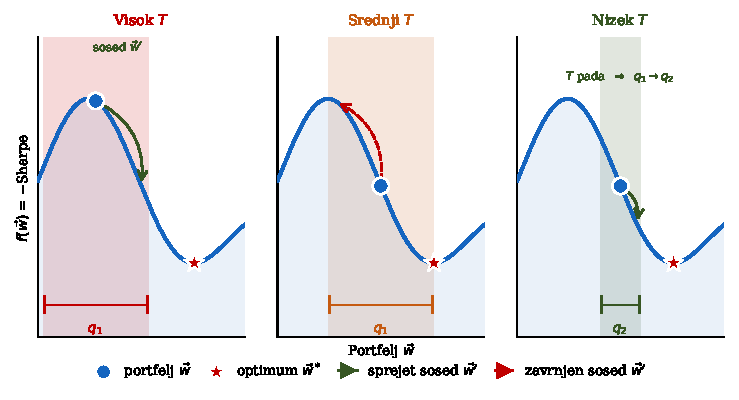
\includegraphics[width=0.85\linewidth]{fig/optimizer_sa_illus.pdf}
    \caption{Poenostavljena ponazoritev delovanja simuliranega ohlajanja v enodimenzionalnem prostoru portfeljev.}
    \label{fig:sa-illus}
\end{figure}

% ============================================================
% IMPLEMENTATION AND EVALUATION
% ============================================================

\clearpage
\section{Implementacija in vrednotenje}\label{sec:impl}

V prejšnjih razdelkih smo ločeno predstavili napovedovanje pričakovanih donosov, ocenjevanje tveganja in reševanje KONP\@. V nadaljevanju te komponente povežemo v naš optimizacijski postopek in postopno vrednotenje ter opišemo njuno programsko izvedbo.

% ------------------------------------------------------------
% SOFTWARE PIPELINE
% ------------------------------------------------------------

\subsection{Programska zasnova}\label{sec:tech}

Pripravo podatkov, učenje modelov, vodenje poskusov in vrednotenje
rezultatov izvajamo v jeziku Python, transformerske modele pa v okolju
PyTorch. Optimizacijski del je implementiran v C++17. Python in C++
komunicirata prek datotek JSON, ki predstavljajo vmesnik med napovednim
in optimizacijskim delom. Celoten tok je prikazan na
Sliki~\ref{fig:pipeline}.

Takšna ločitev omogoča neodvisno izvajanje napovednega in optimizacijskega
dela. JSON-datoteke določajo podatke in parametre, ki se posredujejo
med obema komponentama, ter rezultat optimizacije, ki se vrne v okolje
Python.

% TODO: Opiši vlogo configov, interface za napovedne modele in optimizatorje

\begin{figure}[H]
\centering
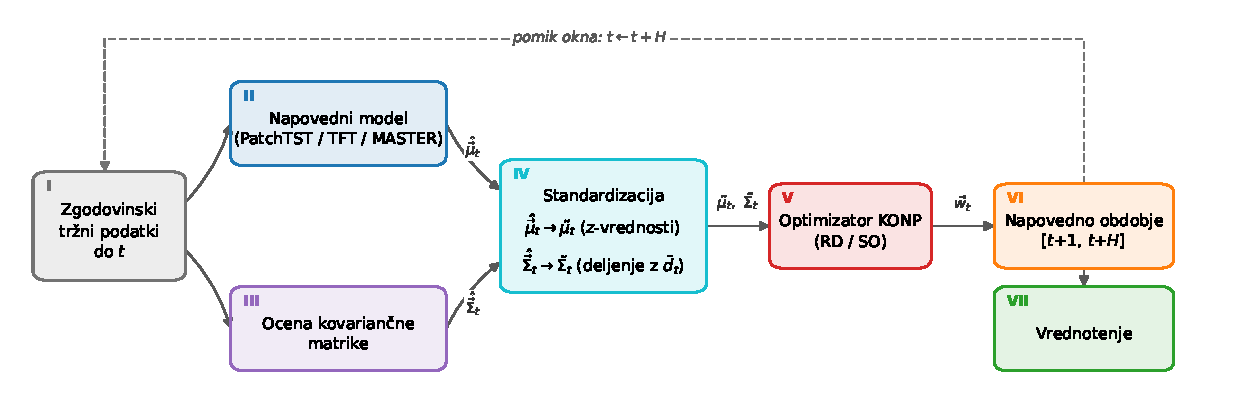
\includegraphics[width=\linewidth]{fig/pipeline.pdf}
\caption{Shema postopka od tržnih podatkov do postopka vrednotenja.}
\label{fig:pipeline}
\end{figure}

% ------------------------------------------------------------
% PIPELINE AND EVALUATION
% ------------------------------------------------------------

\subsection{Potek}\label{sec:forecast-pipeline}\label{sec:optimization-pipeline}\label{sec:eval}

\paragraph{Napoved in optimizacija.}
V korakih~I--IV (Slika~\ref{fig:pipeline}) iz tržnih podatkov, razpoložljivih do odločitvenega trenutka $t$, pripravimo vhodne podatke in ocenimo pričakovane donose $\hat{\vec{\mu}}_t$. Kot referenčni pristop brez nevronskega modela uporabimo zgodovinsko povprečje. Iz zgodovinskih donosov hkrati ocenimo vzorčno kovariančno matriko $\hat{\vec{\Sigma}}_t$, ki je enaka za vse napovedne vire. Napoved in kovarianca se nato uporabita kot vhod v optimizator, ki določi portfeljske uteži $\vec{w}_t$. Prilagoditve napovednih modelov so opisane v razdelkih~\ref{sec:patchtst}, \ref{sec:tft} in \ref{sec:master}, prilagoditve optimizatorjev RD in SO pa v razdelkih~\ref{sec:rd} in~\ref{sec:so}. Pri izračunu variance zaradi učinkovitosti upoštevamo samo aktivna sredstva, s čimer zahtevnost kvadratnega dela zmanjšamo z $O(N^2)$ na $O(K^2)$, ne da bi spremenili vrednost ciljne funkcije.

Pred optimizacijo vse vire pričakovanih donosov $\hat{\vec{\mu}}_t$ prevedemo na skupno brezdimenzionalno skalo. Napovedi presečno standardiziramo v $z$-vrednosti, pri čemer od vsake vrednosti odštejemo presečno povprečje in jo delimo s presečnim standardnim odklonom. Kovariančno matriko $\hat{\vec{\Sigma}}_t$ hkrati normiramo s povprečno vrednostjo njene diagonale, tako da so varianca in kovariance izražene na primerljivi brezdimenzionalni skali. Tako normalizirani $\mu$ in $\Sigma$ uporabimo kot skupna vhoda v optimizator, medtem ko vse naknadno poročane donosnosti in tveganost izračunamo iz nenormaliziranih vrednosti.

\paragraph{Postopno vrednotenje.}
V korakih~V in~VI (Slika~\ref{fig:pipeline}) portfelj $\vec{w}_t$ držimo od $t+1$ do $t+H$, realizirani donos portfelja $r_t^{\mathrm p}$~\eqref{eq:portret} pa izračunamo iz dejanskih prihodnjih cen. Ta postopek postopnega testiranja (angl.\ \emph{walk-forward}) ponavljamo skozi celotno testno obdobje. Pri vsaki odločitvi se napoved, ocena $\hat{\vec{\Sigma}}_t$ in optimizacija izvedejo samo na podlagi do takrat razpoložljivih podatkov; če scenarij zahteva ponovno učenje, se model v predpisanih trenutkih ponovno nauči na takrat razpoložljivih podatkih. Tako prihodnji podatki ne vplivajo na pretekle odločitve.

Časovna okna posameznega koraka so prikazana na Sliki~\ref{fig:proto-schema}. Vhod v napovedni model sestavlja zadnjih $L$ trgovalnih dni pred odločitvenim trenutkom, enako okno pa uporabimo za ujemajočo zgodovinsko osnovno linijo. Vzorčno kovarianco $\hat{\vec{\Sigma}}_t$ ocenimo iz zadnjih $L_{\max}$ trgovalnih dni, kjer je $L_{\max}$ najdaljše pogojno okno med vključenimi modeli, in jo enako uporabimo pri vseh napovednih virih. Portfelj ostane nespremenjen skozi držalno obdobje $H$. Konkretne vrednosti $L$, $L_{\max}$, $H$, pogostost ponovnega učenja in druge nastavitve posameznih benchmarkov so zbrane v Tabeli~\ref{tab:protocols}. Vsa ocenjevalna okna se končajo v odločitvenem trenutku ali pred njim.

\begin{figure}[htbp]
\centering
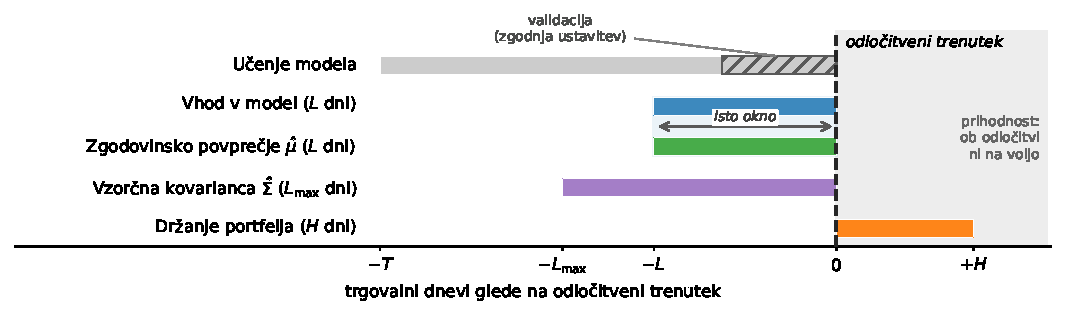
\includegraphics[width=\linewidth]{fig/protocol_schema.pdf}
\caption{Zgradba postopnega vrednotenja za en odločitveni trenutek. Okna ne segajo v osenčeno prihodnost.}
\label{fig:proto-schema}
\end{figure}

% ------------------------------------------------------------
% REPRODUCIBILITY
% ------------------------------------------------------------

\subsection{Nastavitve in ponovljivost}\label{sec:repro}

Vse nastavitve, uporabljene pri eksperimentih, so zbrane v Tabelah~\ref{tab:hparams} in~\ref{tab:repro}. V osnovnih konfiguracijah uporabljamo naključno seme 42 pri TFT in MASTER ter 2021 pri PatchTST; protokolno specifične izjeme in morebitna ponavljanja z več semeni so navedeni neposredno ob posameznem eksperimentu.

\begin{table}[htbp]
\centering
\caption{Ključne nastavitve napovednih modelov in optimizacijskih
algoritmov.}
\label{tab:hparams}
\footnotesize
\begin{tabular}{@{}p{0.18\linewidth}p{0.76\linewidth}@{}}
\textbf{Sklop} & \textbf{Uporabljene nastavitve} \\[3pt]

RD &
velikost roja 200; največ 1500 generacij;
$\alpha_{\mathrm{RD}}=0{,}06$. \\

SO &
$L=2N$; $\alpha_{\mathrm{SO}}=0{,}95$; $v_0=0{,}8$;
$q_1=0{,}005$; $q_2=0{,}001$; $S=5$. \\

TFT &
$k=252$ v večini poskusov in $k=45$ pri Leow All-Weather;
skrita dimenzija 160; 1 glava pozornosti; osip 0,3;
velikost učnega paketa 64; hitrost učenja $10^{-3}$;
največ 100 epoh; potrpežljivost 10; omejitev norme gradienta 0,01. \\

MASTER &
$D=256$; $N_1=4$; $N_2=2$; $\beta=5$;
časovni in presečni osip 0,5; hitrost učenja $10^{-5}$;
največ 100 epoh; potrpežljivost 10. \\

PatchTST &
vhodno okno 336; dolžina časovnega odseka 16; korak 8;
$D=128$; $F=256$; 3 kodirne plasti; 16 glav pozornosti;
osip 0,2; velikost učnega paketa 32; hitrost učenja $10^{-4}$;
največ 100 epoh; potrpežljivost 10; vključena RevIN~\cite{kim2022revin} in
rezidualna pozornost. \\
\end{tabular}
\end{table}

\begin{table}[htbp]
\centering
\caption{Osnovne nastavitve posameznih eksperimentalnih problemov.}
\label{tab:repro}
\scriptsize
\setlength{\tabcolsep}{3pt}
\resizebox{\linewidth}{!}{%
\begin{tabular}{lrrccccccccr}
\textbf{Poskus} &
\textbf{$N$} &
\textbf{$K$} &
\textbf{Uteži} &
\textbf{Učenje} &
\textbf{Test} &
\textbf{Uravnoteževanje} &
\textbf{$H$} &
\textbf{Ponovno učenje} &
\textbf{Optimizator} &
\textbf{Stroški} &
\textbf{$P$} \\[3pt]

Leow All-Weather &
5 & 5 & 0,01--0,40 &
2018--2019 & 2020 &
tedensko & 5 & ob vsaki odločitvi & RD in SO & bruto & 0,05--0,95 (11 točk) \\

Wang S\&P~500 &
494 & 20 & 0,001--1,0 &
2018--2020 & 2021 &
mesečno & 120 & enkrat & RD & bruto & 0,2 \\

Dolgoročni vlagatelj &
61 & 20 & 0,01--0,1 &
2005--2010 & 2011--2024 &
mesečno & 21 & letno & RD & 10 b.\,t. & 0,5 \\
\end{tabular}%
}
\end{table}

Napovedno obdobje $H$ ni lastnost ene same arhitekture, temveč ga določa eksperimentalni scenarij. Enako velja za nabor sredstev, kardinalnost, omejitve uteži, pogostost uravnoteževanja, ponovno učenje in parameter $P$.

{
\renewcommand{\arraystretch}{1.12}

}

% ============================================================
% METRIKE VREDNOTENJA
% ============================================================

\subsection{Mere vrednotenja}\label{sec:metrics}

Ker želimo med različnimi eksperimenti ohraniti čim bolj enotno in hkrati pregledno vrednotenje, pri vseh portfeljskih benchmarkih uporabljamo iste tri skupne metrike: letni donos, letno volatilnost in letni Sharpov količnik. Te metrike so v tabelah vedno navedene najprej in v istem vrstnem redu. Pri zunanjih primerjavah jim po potrebi dodamo le tiste metrike, ki so jih uporabili avtorji raziskav, katerih eksperimentalne scenarije smo uporabili, da lahko naredimo direktno primerjavo z njimi. Napovedni in optimizacijski del pristopa vrednotimo ločeno z manjšim naborom mer, primernim za posamezni problem.

\paragraph{Napovedna kakovost.}

Naj bo $\mathcal{I}_t$ množica sredstev, za katera v času $t$ primerjamo napovedani donos $\hat{\mu}_{i,t}$ z realiziranim donosom $r_{i,t}^{(H)}$ na napovednem obdobje $H$. Napovedno kakovost merimo z informacijskim koeficientom (IC) in rangovnim informacijskim koeficientom (RankIC), ki ju za posamezni časovni korak definiramo kot

\begin{equation}
\label{eq:forecast-correlations}
\begin{aligned}
\mathrm{IC}_t
&=
\operatorname{corr}_{\mathrm P}
\left(
\{\hat{\mu}_{i,t}\}_{i\in\mathcal I_t},
\{r_{i,t}^{(H)}\}_{i\in\mathcal I_t}
\right),
\qquad
&
\mathrm{RankIC}_t
&=
\operatorname{corr}_{\mathrm S}
\left(
\{\hat{\mu}_{i,t}\}_{i\in\mathcal I_t},
\{r_{i,t}^{(H)}\}_{i\in\mathcal I_t}
\right),
\end{aligned}
\end{equation}

kjer $\operatorname{corr}_{\mathrm P}$ označuje Pearsonovo, $\operatorname{corr}_{\mathrm S}$ pa Spearmanovo korelacijo. V rezultatih poročamo povprečje $\mathrm{IC}_t$ in $\mathrm{RankIC}_t$ skozi testno obdobje; višja pozitivna vrednost pomeni močnejšo povezanost med napovedanim in realiziranim donosom, pri čemer RankIC meri predvsem kakovost relativne razvrstitve sredstev.

% ------------------------------------------------------------
% OPTIMIZATION METRIC
% ------------------------------------------------------------

\paragraph{Kakovost optimizacije.}

RD in SO neodvisno od napovednih modelov preverimo na standardnih problemih OR-Library~\cite{beasley1990}. Kardinalno omejeno efektivno fronto primerjamo z objavljeno neomejeno efektivno fronto (USEF) po postopku Changa in sod.~\cite{chang2000}. Standardna odstotna napaka meri relativno oddaljenost najdene rešitve od referenčne fronte; manjša vrednost pomeni kakovostnejšo rešitev, nič pa sovpadanje z referenčno fronto. Ker za posamezno instanco preverimo več vrednosti parametra tveganja, poročamo povprečno in mediansko odstotno napako. Računski čas optimizatorjev poročamo kot spremljevalni podatek o računski zahtevnosti, ne kot mero kakovosti rešitve.

% ------------------------------------------------------------
% COMMON PORTFOLIO METRICS
% ------------------------------------------------------------

\paragraph{Skupne portfeljske metrike.}

Naj bo $\{r_t^{\mathrm p}\}_{t=1}^{T}$ zaporedje realiziranih periodičnih donosov portfelja, $\bar r$ njihovo aritmetično povprečje, $s$ standardni odklon in $p$ število takih obdobij na leto. Kumulativno vrednost portfelja $W_t$, letni donos $R_{\mathrm{letno}}$, letno volatilnost $\sigma_{\mathrm{letno}}$ in letni Sharpov količnik $\mathrm{SR}$ definiramo kot

\begin{equation}
\label{eq:portfolio-common-metrics}
\begin{aligned}
W_t
&=
\prod_{j=1}^{t}(1+r_j^{\mathrm p}),
\qquad
&
R_{\mathrm{letno}}
&=
p\,\bar r,
\\
\sigma_{\mathrm{letno}}
&=
s\sqrt{p},
&
\mathrm{SR}
&=
\frac{\bar r}{s}\sqrt{p}.
\end{aligned}
\end{equation}

Pri dnevnih donosih uporabimo $p=252$, pri tedenskih $p=52$ in pri mesečnih $p=12$. Pri Sharpovem količniku predpostavimo ničelno oziroma zanemarljivo breztvegano donosnost~\cite{sharpe1994}. Višji letni donos je ugodnejši, nižja volatilnost pomeni manjše realizirano tveganje, višji Sharpov količnik pa ugodnejše razmerje med donosom in volatilnostjo. Te tri metrike v vseh naših portfeljskih benchmarkih poročamo v vrstnem redu donos, volatilnost in Sharpe.

\paragraph{Protokolno specifične metrike Wang in sod.}

Pri primerjavi z delom Wang in sod.~\cite{wang2023oneshot} poleg skupnih metrik ohranimo še njihove objavljene portfeljske metrike donosa, tveganja in Sharpovega količnika, saj le tako omogočimo neposredno primerjavo z referenčnimi vrednostmi. Ker njihov način agregiranja rezultatov sledi lastnemu 120-dnevnemu investicijskemu protokolu, te vrednosti v tabeli označimo ločeno od skupnih metrik in jih ne uporabljamo kot nadomestilo za skupni letni donos, volatilnost in Sharpov količnik.

% ------------------------------------------------------------
% SUPPLEMENTARY METRICS
% ------------------------------------------------------------

\paragraph{Promet portfelja.}

Promet portfelja meri velikost spremembe uteži med zaporednima uravnoteženjema in ga za posamezno uravnoteženje izračunamo kot

\begin{equation}
\label{eq:turnover}
\mathrm{TO}_t
=
\sum_{i=1}^{N}
\left|
w_{i,t}-w_{i,t-1}
\right|.
\end{equation}

Višji promet pomeni izrazitejše spremembe sestave portfelja in praviloma več trgovanja. To mero uporabljamo le kot dopolnilno analizo in ne kot glavno merilo uspešnosti benchmarkov.


\newpage
% ============================================================
% REZULTATI
% ============================================================

\section{Rezultati}\label{sec:rezultati}

Vrednotenje je razdeljeno na dve ločeni preverjanji in nato na
pet portfeljskih benchmarkov. Najprej preverimo napovedni del:
ali modeli vsebujejo napovedni signal za prihodnje donose. Nato
preverimo optimizacijski del na standardnih primerih kardinalno
omejenega portfeljskega problema. S tem ločimo morebitne napake
napovednega modela od napak optimizatorja, preden oba dela povežemo
v skupni cevovod.

Glavni del vrednotenja predstavljajo zunanji portfeljski benchmarki.
Trije izhajajo iz predhodnih raziskav, s čimer lahko naš pristop
postavimo v kontekst že objavljenih eksperimentov. Prvi je protokol
Leow in sod.~\cite{leow2021}, ki obravnava portfeljsko odločanje v
obdobju zloma trgov zaradi COVID-19 na petih sredstvih All-Weather.
Drugi sledi podatkovnemu in časovnemu okviru Wang in sod.\
\cite{wang2023oneshot} na 494 sredstvih indeksa S\&P~500 in preverja
primerjavo pristopa \enquote{napovej, nato optimiziraj} z njihovim
enkratnim nevronskim reševalnikom. Tretji je prevzet iz dela Aprea
in Sbaiz~\cite{aprea2026}; zaradi večjega nabora in drugačnega
tržnega okolja ga izvedemo ločeno na sredstvih DJIA in NASDAQ~100.
Ti benchmarki niso replikacije izvornih metod: njihove podatkovne,
časovne in portfeljske nastavitve uporabimo kot zunanji referenčni
okvir, naš napovedni in optimizacijski cevovod pa ostane enak.

Poleg zunanjih benchmarkov vključimo še dolgoročni scenarij, ki ga
oblikujemo sami. Njegov namen ni primerjava z eno samo predhodno
objavljeno metodo, temveč preverjanje, ali se ugotovitve o
napovednem signalu ohranijo tudi pri daljšem obdobju in več
različnih tržnih razmerah. Pri tem dodatno vključimo pasivni indeks
S\&P~500 kot nemodelirano referenco.

Tabela~\ref{tab:protocols} povzema podatkovna obdobja in glavne
nastavitve vseh petih portfeljskih benchmarkov. Podrobnosti
postopnega vrednotenja, časovnih oken, ponovnega učenja in
preprečevanja uhajanja prihodnjih informacij so določene v
razdelku~\ref{sec:eval}; tukaj se osredotočamo na vprašanje, ki ga
posamezen eksperiment preverja, in na dobljene rezultate.

Rezultate zato predstavimo po naslednjem zaporedju: najprej
napovedna kakovost, nato kakovost optimizatorjev, za tem zunanji
benchmarki Leow, Wang ter Aprea in Sbaiz na naborih DJIA in
NASDAQ~100, na koncu pa še dolgoročni scenarij in dopolnilna analiza
stabilnosti portfeljev.

\begin{table}[htbp]
\centering
\small
\caption{Nastavitve postopnega vrednotenja po benchmarkih ($H$ = napovedno obdobje, $K$ = kardinalnost).}
\label{tab:protocols}
\begin{tabular}{llllrrr}
\hline
Benchmark & Učenje & Preizkus & Obnovitev & $H$ & $K$ & Val. \\
\hline
Leow All-Weather   & 2018--2019 & jan.--apr.~2020 & ob vsaki odločitvi & 5   & 5  & 63 \\
Wang S\&P~500      & 2018--2020 & 2021            & enkratna           & 120 & 20 & 120 \\
Aprea DJIA         & 2007--2015 & 2016--2020      & letna              & 21  & 10 & 126 \\
Aprea NASDAQ~100   & 2007--2015 & 2016--2020      & letna              & 21  & 10 & 126 \\
Dolgoročni vlagatelj & 2005--2010 & 2011--2024    & letna              & 21  & 20 & 126 \\
\hline
\end{tabular}
\end{table}

% ------------------------------------------------------------
% FORECAST QUALITY
% ------------------------------------------------------------

\subsection{Napovedna kakovost na standardnem protokolu}\label{sec:pred}

Preden vključimo optimizator, preverimo, ali modeli sploh vsebujejo koristni napovedni signal. Vprašanje je preprosto: ali napovedi transformerjev o prihodnjih donosih sploh korelirajo z dejansko realiziranimi donosi?

Testni scenarij: 494 sredstev indeksa S\&P~500, učenje 2018--2020, preizkus v letu 2021, napovedno obdobje pet dni. Vsak dan napovedujemo donose za vsa sredstva hkrati in primerjamo napovedi z realiziranimi vrednostmi. Ker nas zanima presečna kakovost (katera sredstva model pravilno razvrsti glede na donos), merimo IC in RankIC, ki sta definirani v razdelku~\ref{sec:metrics}. Optimizator tu sploh ni vključen.

\begin{table}[htbp]
\centering
\caption{Napovedna kakovost na presečnem protokolu (S\&P~500, učenje 2018--2020, preizkus 2021, horizont pet dni).}
\label{tab:pred}
\begin{tabular}{lrr}
\hline
Vir napovedi & IC & RankIC \\
\hline
Zgodovinski & $-0{,}0284$ & $-0{,}0213$ \\
MASTER      & $+0{,}0014$ & $-0{,}0009$ \\
TFT         & $+0{,}0405$ & $+0{,}0363$ \\
PatchTST    & $-0{,}0031$ & $+0{,}0006$ \\
\hline
\end{tabular}
\end{table}

Rezultate povzema Tabela~\ref{tab:pred}. Zgodovinski pristop v letu 2021 doseže negativni IC in RankIC: napovedi na podlagi preteklih povprečij ne korelirajo z realiziranimi donosi. Vsi trije transformerji presežejo to izhodišče. TFT je edini z izrazito pozitivnim IC ($+0{,}04$) in RankIC ($+0{,}04$), kar pomeni, da njegove napovedi merljivo korelirajo s kasnejšimi donosi. MASTER in PatchTST se gibljeta blizu nič -- napovedi niso sistemično napačne, a tudi ne zanesljivo pravilne.

Ta preizkus ne določi vrstnega reda modelov pri sestavi portfelja, saj dobra presečna napoved ni nujno enaka dobri portfeljski uspešnosti. Pokaže pa, da transformerji vsebujejo boljši signal od gole zgodovine. Naslednji eksperimenti preverijo, ali se ta prednost prenese v portfeljske donose.

% ------------------------------------------------------------
% OPTIMIZER QUALITY
% ------------------------------------------------------------

\subsection{Kakovost optimizatorjev na standardnih primerih}\label{sec:orlib}

Preden vključimo napovedne modele, preverimo, ali optimizator pravilno rešuje kardinalno omejeni problem povprečja in variance. Vprašanje je: ali RD in SO najdeta portfelje blizu optimalne efektivne fronte?

Testni scenarij: pet standardnih primerov zbirke OR-Library~\cite{beasley1990}: Hang Seng (31 sredstev), DAX~100 (85), FTSE~100 (89), S\&P~100 (98) in Nikkei (225). Za vsak primer izračunamo kardinalno omejeno efektivno fronto pri 50 vrednostih parametra tveganja ($K=10$, $\varepsilon_i=0{,}01$, $\delta_i=1$) in jo primerjamo z objavljeno neomejeno fronto (USEF) po postopku Changa in sod.~\cite{chang2000}. $\hat{\vec{\mu}}$ in $\hat{\vec{\Sigma}}$ vzamemo neposredno iz referenčnih podatkovnih datotek, da napovedni model ne vpliva na rezultat.

\begin{table}[htbp]
\centering
\begin{minipage}[t]{\linewidth}
\vspace{0pt}
\centering
\caption{Standardna odstotna napaka (\%) kardinalno omejene fronte glede na USEF na primerih OR-Library.}
\label{tab:orlib}
\footnotesize
\begin{tabular}{lrrrr}
\hline
 & \multicolumn{2}{c}{RD} & \multicolumn{2}{c}{SO} \\
Instanca ($N$) & povpr. & med. & povpr. & med. \\
\hline
Hang Seng (31)  & 1,28 & 1,26 & 1,12 & 1,22 \\
DAX 100 (85)    & 2,93 & 2,66 & 3,45 & 2,61 \\
FTSE 100 (89)   & 2,03 & 1,29 & 1,63 & 1,08 \\
S\&P 100 (98)   & 2,93 & 1,61 & 2,51 & 1,18 \\
Nikkei (225)    & 1,96 & 1,33 & 0,61 & 0,60 \\
\hline
Povprečje        & 2,23 & 1,63 & 1,86 & 1,34 \\
\hline
\end{tabular}
\end{minipage}
\end{table}

\begin{figure}[htbp]
\centering
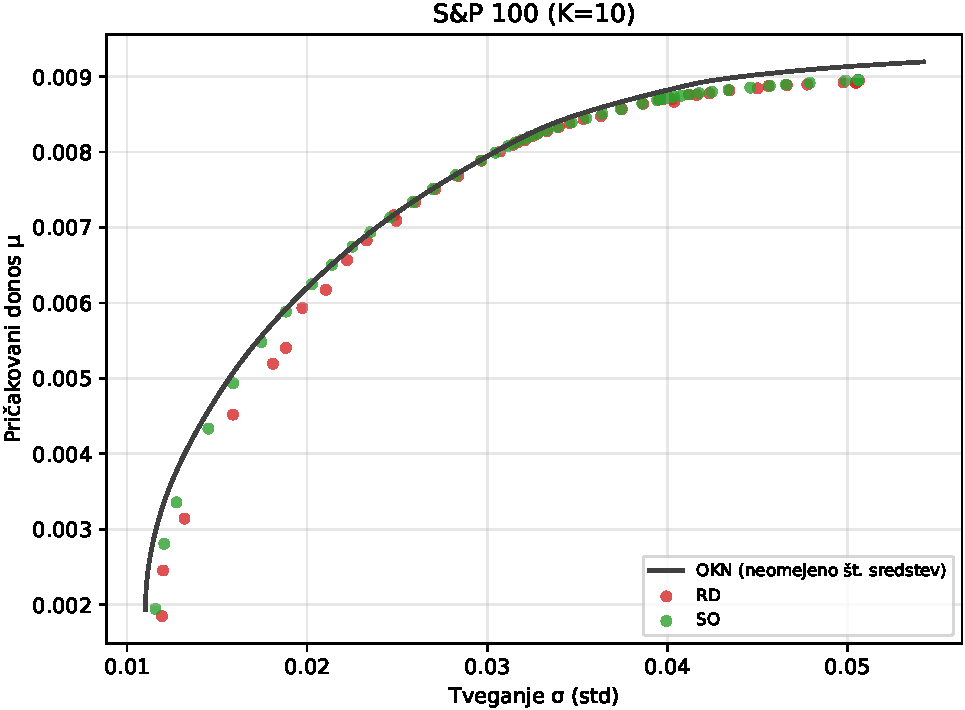
\includegraphics[height=\figheight]{fig/orlib_frontier_sp100.pdf}
\caption{Kardinalno omejena fronta na primeru S\&P~100: RD in SO v primerjavi z neomejeno fronto (USEF); vsaka točka predstavlja eno vrednost parametra tveganja.}
\label{fig:orlib}
\end{figure}

Tabela~\ref{tab:orlib} kaže, da oba optimizatorja dosegata rešitve blizu objavljene neomejene fronte. Povprečna odstotna napaka je pri večini primerov pod $3\,\%$, mediana pa je pri obeh algoritmih v povprečju nižja od $2\,\%$. SO ima nekoliko nižjo skupno povprečno in mediansko napako kot RD, vendar prednost ni enaka pri vseh instancah.

Slika~\ref{fig:orlib} rezultat ponazori na primeru S\&P~100, kjer se točke obeh kardinalno omejenih postopkov skozi večji del razpona tesno približajo neomejeni fronti. To zmanjšuje verjetnost, da bi bile razlike med napovednimi modeli v nadaljnjih poskusih predvsem posledica očitno nekakovostnega optimizacijskega postopka.

Računska zahtevnost obeh optimizatorjev je pri teh problemih majhna: posamezno reševanje traja med $0{,}02$ in $0{,}26\,$s, celoten pregled petih primerov s po 50 vrednostmi parametra tveganja pa se zaključi v manj kot minuti.

% ------------------------------------------------------------
% LEOW
% ------------------------------------------------------------

\subsection{Zunanja primerjava z delom Leow in sod.}\label{sec:leow}

Leow in sod.~\cite{leow2021} razširijo klasično optimizacijo portfelja z razpoloženjem, pridobljenim iz družbenih omrežij. Besedilne objave obdelajo z modelom BERT in iz njih izluščijo razpoloženjski signal, ki ga vključijo v kriterij optimizacije skupaj z genetskim algoritmom. Njihova najboljša metoda (SAW) v kriznem obdobju COVID-19 doseže Sharpov količnik $2{,}14$.

\textbf{Testni scenarij.} Prevzamemo njihovo časovno delitev (januar--april 2020, 13 tedenskih odločitev). Namesto razpoloženjskega signala v postopek vstavimo naše napovedi $\hat{\vec{\mu}}$, zato gre za primerjavo napovednega in optimizacijskega pristopa v sorodnem protokolu, ne za reprodukcijo njihovega signala. Testiramo njihov petsredstveni nabor All-Weather (VTI, TLT, IEF, GLD, DBC; kardinalnost $K{=}5$) -- edini nabor, za katerega Leow in sod.\ poročajo številčne rezultate (njihovi tabeli~4 in~6). Sektorski nabor SPDR v njihovem delu nastopa le kot slika brez poročanih mer in ga zato ne uporabljamo za primerjavo. Vprašanje je, ali naš transformerski signal v krizi dosega primerljive rezultate z njihovim razpoloženjskim pristopom.

Ker isti $P$ pri različnih virih $\hat{\vec{\mu}}$ pomeni različno realizirano tveganje, vsak model poročamo pri tistem $P$, pri katerem je njegova realizirana letna volatilnost najbližja volatilnosti ujemajoče zgodovinske osnovne linije; s tem so donos in Sharpov količnik primerjani pri enakem realiziranem tveganju. Vsak transformer je primerjan z lastno osnovno linijo: \enquote{Zgodovinski\,($L$\,dni)} označuje vzorčno povprečje čez $L$ trgovalnih dni, kjer $L$ ustreza pogojnemu oknu tistega modela (PatchTST: $L{=}\LeowAWWindowPatchTST$, TFT: $L{=}\LeowAWWindowTFT$). Ta konvencija in oznaka veljata za vse portfeljske tabele v nadaljevanju. Stolpec \enquote{Čas učenja} je skupni čas učenja čez vse ponovitve in semena (\LeowAWTrainNTFT{} učenj na model); zgodovinski pristop je označen z \enquote{--}.

\begin{table}[htbp]
\centering
\caption{Portfeljska uspešnost v protokolu Leow in sod.~\cite{leow2021} (jan.--apr.~2020, \LeowAWDecisions{} tedenskih odločitev, nabor All-Weather, optimizator RD, bruto). Referenčne vrednosti iz njihove Tabele~6.}
\label{tab:leow}
\scriptsize
\begin{tabular}{llrrrr}
\hline
Nabor & Metoda & Donos & Volatilnost & Sharpe & Čas učenja \\
\hline
All-Weather & Leow: SPY (pasivno)   & $-65{,}4\,\%$ & $55{,}1\,\%$ & $-1{,}65$ & -- \\
All-Weather & Leow: CRB (pasivno)   & $-8{,}5\,\%$  & $17{,}8\,\%$ & $-0{,}41$ & -- \\
All-Weather & Leow: MPT (Markowitz) & $+13{,}6\,\%$ & $18{,}0\,\%$ & $+0{,}80$ & -- \\
All-Weather & Leow: SAW (najboljši) & $+53{,}9\,\%$ & $21{,}2\,\%$ & $+2{,}14$ & -- \\
All-Weather & Zgodovinsko povprečje\,(45\,dni) & $29{,}6\,\%$ & $20{,}9\,\%$ & $1{,}42$ & -- & -- & 68\,ms & 17\,ms \\
All-Weather & Zgodovinsko povprečje\,(64\,dni) & $11{,}2\,\%$ & $24{,}4\,\%$ & $0{,}46$ & -- & -- & 66\,ms & 16\,ms \\
All-Weather & PatchTST & $14{,}6\,\%$ & $22{,}7\,\%$ & $0{,}64$ & 65 & 17{,}0\,s & 68\,ms & 17\,ms \\
All-Weather & TFT & $28{,}6\,\%$ & $22{,}2\,\%$ & $1{,}29$ & 65 & 18{,}6\,s & 67\,ms & 17\,ms%
\\
\hline
\end{tabular}
\end{table}

\textbf{Rezultati -- All-Weather.} Ker vsak model bere svoje pogojno okno, ni ene same \enquote{zgodovinske} primerjalne vrednosti: vzorčno povprečje čez \LeowAWWindowPatchTST{} dni doseže Sharpe $\LeowAWHistoricalPatchTST$ (letni donos \LeowAWHistoricalPatchTSTRet{}), čez \LeowAWWindowTFT{} dni pa le $\LeowAWHistoricalTFT$ (\LeowAWHistoricalTFTRet{}). Že ta razlika -- devetnajst dodatnih dni zgodovine prepolovi Sharpov količnik -- pokaže, da je dolžina okna v tem obdobju enako pomembna kot izbira napovednika. TFT doseže Sharpe $\LeowAWTFT$ (\LeowAWTFTRet{}) in tako za $\LeowAWMarginTFT$ jasno prekaša svojo ujemajočo osnovno linijo, medtem ko PatchTST s Sharpom $\LeowAWPatchTST$ (\LeowAWPatchTSTRet{}) svoji osnovni liniji občutno podleže ($\LeowAWMarginPatchTST$). TFT s Sharpom $\LeowAWTFT$ preseže tudi Leowov MPT z maksimizacijo Sharpovega količnika ($+0{,}80$) in se približa njihovemu modelu z minimizacijo volatilnosti ($+1{,}51$), ne doseže pa najvišje vrednosti Leow in sod.\ ($+2{,}14$, model SAW z maksimizacijo donosa); PatchTST s Sharpom $\LeowAWPatchTST$ v tej ponovitvi ne doseže niti njihovega MPT.

Rezultate je treba brati previdno. Izhajajo iz le \LeowAWDecisions{} tedenskih odločitev v izjemno kratkem kriznem obdobju, zato so občutljivi na posamezne realizirane donose in na podrobnosti učenja. Kako občutljivi, kaže naslednja primerjava z zgodnejšo ponovitvijo istega protokola: zgolj sprememba dolžine validacijskega okna za zgodnje ustavljanje (pri TFT skupaj s spremembo potrpežljivosti), torej učinkovitostna nastavitev, ki ne spremeni niti podatkov niti arhitekture, je Sharpov količnik TFT premaknila z $+0{,}21$ na $\LeowAWTFT$, pri PatchTST pa v nasprotno smer, z $+1{,}09$ na $\LeowAWPatchTST$. Velik del razpona med modeloma v tem obdobju je torej šum pri izbiri ustavitvene točke učenja in ne stabilna napovedna vsebina; primerjava je zato zgolj usmeritvena, vrstni red modelov pa se lahko z drugačno nastavitvijo zgodnjega ustavljanja ponovno obrne.

Razlike med modeloma v tem naboru niso skladne z njihovo napovedno kakovostjo -- kar je samo po sebi pomembna ugotovitev. PatchTST doseže pozitiven presečni $R^2$ ($+0{,}018$; $R^2_{\mathrm{OS}} = +0{,}029$ proti svoji osnovni liniji pri $-0{,}012$), kar je edini pozitivni absolutni $R^2$ med vsemi štirimi viri v tem naboru -- pa vendar je njegov portfeljski Sharpe najnižji med transformerji. TFT ostane pri negativnem absolutnem $R^2$ ($-0{,}009$), a rahlo prekaša svojo osnovno linijo ($R^2_{\mathrm{OS}} = +0{,}006$). Portfeljski izid se torej obrne glede na presečno napovedno kakovost: boljši $R^2$ (PatchTST) ne prinese boljšega Sharpovega količnika. To je skladno z ugotovitvijo razdelka~\ref{sec:pred}, da dobra presečna korelacija ne zagotavlja dobre portfeljske uspešnosti; slednjo dodatno določata razporeditev uteži in odziv optimizatorja na velikost napovedanih donosov (razdelek~\ref{sec:whytft}). Ob \LeowAWDecisions{} odločitvah gre za usmeritveno in ne statistično značilno ugotovitev.

Gibanje vrednosti posameznih portfeljev skozi to obdobje prikazuje Slika~\ref{fig:leow}. Skupna ugotovitev je, da visok ali nizek rezultat posameznega napovednika v tem kratkem obdobju ne odraža splošne superiornosti modela. Obdobje obsega le 13 tedenskih odločitev znotraj enega samega zloma, zato rezultate beremo zgolj ekonomsko in usmeritveno, brez statistične značilnosti.

\begin{figure}[htbp]
\centering
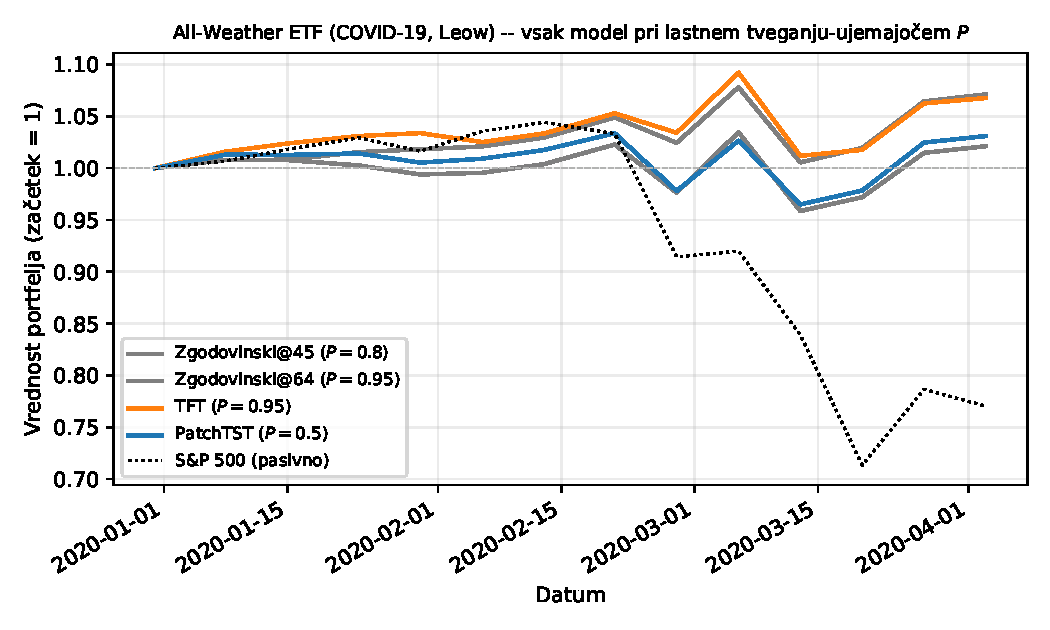
\includegraphics[height=\figheight]{fig/equity_all_leow_allweather.pdf}
\caption{Gibanje vrednosti portfelja All-Weather med COVID-19 zlomom (protokol Leow in sod., bruto). Vsak model je prikazan pri ujemajočem $P$ iz Tabele~\ref{tab:leow}.}
\label{fig:leow}
\end{figure}


% ------------------------------------------------------------
% WANG
% ------------------------------------------------------------

\subsection{Zunanja primerjava z delom Wang in sod.}\label{sec:wang}

Wang in sod.~\cite{wang2023oneshot} predlagajo enkratni nevronski reševalnik CardNN-GS za kardinalno omejeni portfeljski problem. Namesto ločenega napovednega in optimizacijskega koraka reševalnik oba združi v enoten model z diferenciabilno plastjo optimalnega transporta, ki neposredno maksimizira Sharpov količnik. Kot primerjalno metodo vključijo tudi pristop \enquote{napovej, nato optimiziraj}: LSTM oceni pričakovane donose, Gurobi pa na podlagi teh ocen poišče optimalne uteži. Ta pristop je strukturno najbližji našemu.

\textbf{Testni scenarij.} Prevzamemo njihov podatkovni nabor: 494 sredstev iz indeksa S\&P~500, leto 2021 kot testno obdobje, 120-dnevni horizont odločanja, kardinalnost $K{=}20$. Kovariančno matriko fiksiramo na učnem obdobju 2018--2020; to je odstopanje od njihovega protokola, kjer $\hat{\vec{\Sigma}}$ ni fiksna, temveč jo za vsako odločitev izračunajo iz napovedanih prihodnjih donosov modela LSTM\@. Naš pristop take napovedane $\hat{\vec{\Sigma}}$ nima, zato uporabimo vzorčno oceno iz učnega obdobja, ki v testno obdobje ne pogleda. Ker Wang in sod.\ neposredno maksimizirajo Sharpov količnik, naša ciljna funkcija povprečje--varianca pri $P{=}0{,}5$ temu ni enakovredna -- primerjava je smiselna na ravni Sharpa, ki tveganje že upošteva. Vprašanje je, ali metahevristična optimizacija s standardno ciljno funkcijo doseže primerljivo kakovost kot specializirani nevronski reševalci.

Dve opombi pred branjem Tabele~\ref{tab:wang}: Wang in sod.\ Sharpov količnik računajo z netvegano mero $3\,\%$, mi pa brez nje, zato so naše vrednosti v tem stolpcu za ~$0{,}15$ ugodnejše. Poleg tega so standardni odkloni Sharpovih količnikov v tem protokolu večji od samih vrednosti (od \WangSharpeStdMin{} do \WangSharpeStdMax), zato tabela dopušča le umestitev v razred, ne razvrstitve med posameznimi modeli.

\begin{table}[htbp]
\centering
\caption{Primerjava z delom Wang in sod.~\cite{wang2023oneshot} (S\&P~500 2021, 120-dnevna okna, $K{=}20$, optimizator RD). Referenčne vrednosti iz njihove Tabele~3 in Slike~5.}
\label{tab:wang}
\begin{tabular}{lrrrr}
\hline
Metoda & Donos & Tveganje & Sharpe & Čas učenja \\
\hline
Wang: zgodovinski (Gurobi)       & 0{,}139 & 0{,}162 & $0{,}673$ & -- \\
Wang: napovej-nato (LSTM+Gurobi) & 0{,}241 & 0{,}195 & $1{,}082$ & -- \\
Zgodovinsko povprečje\,(67\,dni) & $22{,}3\,\%$ & $22{,}5\,\%$ & $0{,}86$ & -- & -- & 2{,}0\,s & 1{,}6\,s \\
Zgodovinsko povprečje\,(271\,dni) & $27{,}8\,\%$ & $25{,}4\,\%$ & $1{,}08$ & -- & -- & 2{,}0\,s & 1{,}6\,s \\
Zgodovinsko povprečje\,(336\,dni) & $35{,}8\,\%$ & $25{,}6\,\%$ & $1{,}41$ & -- & -- & 2{,}0\,s & 1{,}6\,s \\
MASTER & $29{,}6\,\%$ & $23{,}1\,\%$ & $1{,}12$ & 1 & 33{,}7\,min & 2{,}0\,s & 1{,}6\,s \\
PatchTST & $36{,}3\,\%$ & $22{,}7\,\%$ & $1{,}64$ & 1 & 1{,}8\,min & 2{,}0\,s & 1{,}6\,s \\
TFT & $40{,}2\,\%$ & $24{,}6\,\%$ & $1{,}79$ & 1 & 1{,}04\,h & 2{,}1\,s & 1{,}5\,s%
\\
Wang: napovej-in (CardNN-GS)     & 0{,}400 & 0{,}188 & $1{,}968$ & -- \\
\hline
\end{tabular}
\end{table}

\textbf{Rezultati.} Naš pristop se objavljenim metodam dobro primerja. TFT doseže Sharpe $\WangTFT$, tik pred njim PatchTST z $\WangPatchTST$; oba se uvrstita med Wangov pristop \enquote{napovej, nato optimiziraj} (LSTM+Gurobi, $1{,}08$) in njihov enkratni nevronski reševalnik CardNN-GS ($1{,}97$), ki neposredno maksimizira Sharpov količnik. Komercialni Gurobi pri njih uporabljata prav primerjalni metodi (zgodovinska in \enquote{napovej, nato optimiziraj}), medtem ko ga CardNN-GS nadomesti. Pri tem je naš letni donos ($\WangTFTRet$) skoraj enak CardNN-GS ($0{,}400$), a ob občutno višjem realiziranem tveganju ($\WangTFTRisk$ proti $0{,}188$): del razlike v Sharpovem količniku torej ni posledica boljših napovedi, temveč večje izpostavljenosti.

Dva rezultata je treba navesti odkrito. Prvič, MASTER s Sharpom $\WangMASTER$ ostaja najšibkejši od treh transformerjev v tem protokolu, čeprav svojo ujemajočo osnovno linijo ($\WangHistoricalMASTER$) prekaša le za $\WangMarginMASTER$; njegova prednost pred zgodovino je torej postranska in bistveno manjša kot pri TFT in PatchTST\@. Drugič, sama zgodovinska osnovna linija čez \WangWindowPatchTST{} dni doseže Sharpe $\WangHistoricalPatchTST$ in s tem prekaša Wangov LSTM+Gurobi ($1{,}08$) -- brez vsakršnega napovednega modela. Razpon osnovnih linij ($\WangHistoricalMASTER$, $\WangHistoricalTFT$, $\WangHistoricalPatchTST$ pri \WangWindowMASTER, \WangWindowTFT{} in \WangWindowPatchTST{} dneh) je primerljiv z razponom med modeli, kar pomeni, da dolžina okna v tem protokolu opravi približno toliko dela kot izbira napovednika.

Skupna ugotovitev je zato zadržana: odprtokodna metahevristična optimizacija s standardno ciljno funkcijo povprečje--varianca dosega kakovost v razredu specializiranih nevronskih reševalcev brez potrebe po komercialni infrastrukturi, vendar protokol s sedmimi odločitvami in $83\,\%$ prekrivanjem obdobij držanja (kar ustreza približno dvema neodvisnima opazovanjema) ne dopušča razvrstitve med posameznimi napovedniki.

% ------------------------------------------------------------
% APREA DJIA
% ------------------------------------------------------------

\subsection{Zunanja primerjava z delom Aprea in Sbaiz: DJIA}\label{sec:aprea-djia}

Aprea in Sbaiz~\cite{aprea2026} predlagajo globoko naučen pristop k izbiri portfelja, ki namesto variance kot mere tveganja minimizira agregiran $\Delta$CoVaR (sistemsko tveganje, ocenjeno z LSTM) ob dodatnih omejitvah ESG, prometa in minimalnega donosa. Nastali nekonveksni problem rešujejo z izboljšanim rojenjem delcev, pri katerem parametre roja ($w$, $c_1$, $c_2$) sproti prilagaja nevronska mreža, omejitve pa obravnavajo s projekcijo na proračunsko simpleks in kazensko funkcijo. Njihova ciljna funkcija in omejitve so torej bistveno drugačne od našega povprečje--variančnega kriterija, zato gre za primerjavo metod na skupnih naknadno izračunanih merah (Sharpov količnik, letni donos), ne za replikacijo; skupna pa je izbira rojenja delcev kot reševalnika.

\textbf{Testni scenarij.} Prevzamemo njihov nabor 28 sredstev indeksa DJIA (poravnan z njihovim investicijskim naborom na presečni datum 31.\,12.\,2020, rekonstruiran iz javno dostopnih cen) in njihovo časovno shemo: učenje na obdobju 2007--2015, mesečno odločanje v obdobju 2016--2020 (60 razporeditev; njun $T_f{=}59$ šteje ponovna uravnoteženja po začetni razporeditvi) in $w_{\max}{=}0{,}2$ (zgornja meja uteži, skladna z eno od dveh mej Aprea in sod.). Kardinalnost $K{=}10$ je \emph{naš} dodatek: njun model kardinalne omejitve ne vsebuje -- njune omejitve so proračunska, intervalna ($x_i \in [l_i,u_i]$), ESG, prometna in minimalni donos, brez binarnih spremenljivk. Število pozicij pri njih ni nastavitev, temveč posledica intervalne meje: zadnja vrstica njunih tabel~7 in~8 poroča \emph{povprečno} število sredstev z neničelno utežjo zunaj vzorca, in to je $10$ pri $u_i{=}0{,}2$ ter $16$ pri $u_i{=}0{,}06$, torej $\lfloor 1/u_i \rfloor$. Naš $K{=}10$ pri $w_{\max}{=}0{,}2$ tako eksplicitno predpiše prav tisto število pozicij, ki pri njiju nastane samo od sebe. Njihova omejitev prometa ($\leq 0{,}2$ na odločitev), omejitev ESG in kriterij minimalnega donosa v našem pristopu niso implementirani, zato je neposredna primerjava s to referenco zgolj usmeritvena.



\begin{table}[htbp]
\centering
\caption{Primerjava z delom Aprea in Sbaiz~\cite{aprea2026} na naboru sredstev DJIA (28 sredstev, 2016--2020, 60 mesečnih odločitev, $K{=}10$, $P{=}0{,}5$, optimizator RD, bruto).}
\label{tab:apreadjia}
\begin{tabular}{lrrr}
\hline
Metoda & Donos & Volatilnost & Sharpe \\
\hline
Zgodovinski\,(67\,dni)  & $14{,}1\,\%$ & $15{,}3\,\%$ & 0,75 \\
Zgodovinski\,(271\,dni) & $12{,}4\,\%$ & $15{,}5\,\%$ & 0,64 \\
Zgodovinski\,(336\,dni) & $14{,}8\,\%$ & $15{,}5\,\%$ & 0,80 \\
MASTER   & $16{,}3\,\%$ & $17{,}2\,\%$ & 0,76 \\
PatchTST & $19{,}3\,\%$ & $15{,}4\,\%$ & 1,09 \\
TFT      & $16{,}9\,\%$ & $16{,}9\,\%$ & 0,79 \\
\hline
Aprea in Sbaiz: B$^+$ ($p{=}1\,\%$, $u_i{=}0{,}2$) & $20{,}8\,\%$ & $5{,}0\,\%$\footnotemark[1] & $1{,}21$\footnotemark[2] \\
\hline
\end{tabular}
\footnotetext[1]{Objavljena kot mesečna periodna volatilnost ($5{,}01\,\%$), ni neposredno primerljiva z letno volatilnostjo v zgornjih vrsticah.}
\footnotetext[2]{Letno normalizirana vrednost njihovega mesečnega periodnega Sharpa ($0{,}3502 \times \sqrt{12}$); minimizira $\Delta$CoVaR, ne variance, zato je primerjava zgolj usmeritvena.}
\end{table}

\textbf{Rezultati.} Rezultate zbira Tabela~\ref{tab:apreadjia}. Na tem naboru vsi trije transformerji presežejo svojo ujemajočo zgodovinsko osnovno linijo. PatchTST doseže najvišji Sharpe ($1{,}09$ proti $0{,}80$ za osnovno linijo čez 336 dni) in edini preseže tudi Apreovo referenco ($1{,}21$ letno normalizirano), čeprav ob občutno višji volatilnosti -- njihov model eksplicitno minimizira tveganje (sistemsko, ne variančno), naš pa ga uravnoteži z donosom pri $P{=}0{,}5$. TFT ($0{,}79$ proti $0{,}64$) in MASTER ($0{,}76$ proti $0{,}75$, komaj) prav tako presežeta svoji osnovni liniji, a z manjšo razliko; MASTER je tu na robu. Noben od treh ne doseže Apreove referenčne volatilnosti niti pri sami metodologiji ($\Delta$CoVaR proti varianci, brez omejitve prometa), zato branje te tabele ostaja usmeritveno.

% ------------------------------------------------------------
% APREA NASDAQ100
% ------------------------------------------------------------

\subsection{Zunanja primerjava z delom Aprea in Sbaiz: NASDAQ~100}\label{sec:aprea-nasdaq}

Isti protokol Aprea in Sbaiz~\cite{aprea2026} ponovimo na njihovem večjem naboru 54 sredstev indeksa NASDAQ~100 (poravnanem z njihovim polnozgodovinskim naborom), da preverimo, ali se ugotovitve iz razdelka~\ref{sec:aprea-djia} prenesejo na širši, bolj tehnološko nagnjen nabor sredstev. Nastavitve (obdobje, $K{=}10$, $w_{\max}{=}0{,}2$, 60 mesečnih odločitev) so sicer enake kot pri DJIA.



\begin{table}[htbp]
\centering
\caption{Primerjava z delom Aprea in Sbaiz~\cite{aprea2026} na naboru NASDAQ~100 (54 sredstev, 2016--2020, 60 mesečnih odločitev, $K{=}10$, $P{=}0{,}5$, optimizator RD, bruto).}
\label{tab:aprealndaq}
\begin{tabular}{lrrr}
\hline
Metoda & Donos & Volatilnost & Sharpe \\
\hline
Zgodovinski\,(67\,dni)  & $28{,}0\,\%$ & $21{,}7\,\%$ & 1,03 \\
Zgodovinski\,(271\,dni) & $28{,}3\,\%$ & $23{,}3\,\%$ & 0,94 \\
Zgodovinski\,(336\,dni) & $30{,}6\,\%$ & $23{,}9\,\%$ & 1,00 \\
MASTER   & $27{,}0\,\%$ & $18{,}4\,\%$ & 1,23 \\
PatchTST & $30{,}9\,\%$ & $24{,}9\,\%$ & 0,96 \\
TFT      & $18{,}9\,\%$ & $22{,}7\,\%$ & 0,55 \\
\hline
Aprea in Sbaiz: B$^+$ ($p{=}1\,\%$, $u_i{=}0{,}2$) & $22{,}9\,\%$ & $6{,}3\,\%$\footnotemark[1] & $1{,}08$\footnotemark[2] \\
\hline
\end{tabular}
\footnotetext[1]{Objavljena kot mesečna periodna volatilnost, ni neposredno primerljiva z letno.}
\footnotetext[2]{Letno normalizirana vrednost njihovega mesečnega periodnega Sharpa.}
\end{table}

\textbf{Rezultati.} Rezultate zbira Tabela~\ref{tab:aprealndaq}. Na tem večjem, bolj tehnološko nagnjenem naboru se vrstni red modelov obrne glede na DJIA\@. MASTER je tu edini, ki jasno preseže svojo osnovno linijo ($1{,}23$ proti $1{,}03$ čez 67 dni) in edini preseže tudi Apreovo referenco ($1{,}08$ letno normalizirano). PatchTST ostane praktično na ravni svoje osnovne linije ($0{,}96$ proti $1{,}00$, neznatno nižje). TFT je edini model, ki v tem naboru izrazito zaostane za svojo osnovno linijo ($0{,}55$ proti $0{,}94$) -- v nasprotju z njegovo vlogo v Leow All-Weather in dolgoročnem scenariju (razdelek~\ref{sec:longterm}), kjer osnovno linijo presega. Diagnostika kaže, da gre pri TFT deloma za arhitekturno omejitev pri tem večjem naboru: TFT za razliko od MASTER nima presečne (medsredstvene) pozornosti in torej svoje kapacitete ne prilagaja velikosti nabora, kar je pri 54 sredstvih izrazitejša ovira kot pri 28 (DJIA) ali petih (Leow). Rezultat je zato treba brati kot opozorilo, da uspešnost posameznega transformerja ni univerzalna lastnost modela, temveč je odvisna tudi od velikosti in narave nabora sredstev -- kar je skladno s skupno ugotovitvijo tega dela, da noben posamezni napovednik ne dominira dosledno prek vseh benchmarkov, medtem ko je v vsakem benchmarku vsaj eden, ki svojo zgodovinsko osnovno linijo preseže (tu MASTER).

% ------------------------------------------------------------
% LONG-TERM INVESTOR
% ------------------------------------------------------------

\subsection{Praktični scenarij: dolgoročni vlagatelj}\label{sec:longterm}

Predhodne primerjave preverijo optimizacijski pristop s postopnim vrednotenjem na primerih obstoječih raziskav. Kot zadnji korak izvedemo scenarij, ki ga sami oblikujemo za preverbo dolgoročnega vedenja: ali transformerski signal ostaja koristen prek daljšega obdobja z večimi tržnimi razmerami, ne le v kratkem kriznem oknu?

\textbf{Testni scenarij.} Testiramo na naboru ameriških sredstev v obdobju 2011--2024 z letnim preučevanjem (12 odločitev). Ker scenarij ni vezan na referenčno študijo, referenčna točka je naš lasten zgodovinski pristop in pasivni indeks S\&P~500 (dodan kot ločena, nemodelirana referenca; ker nima prometa, velja bruto = neto). Opozorilo: nabor vsebuje samo sredstva, ki so preživela celotno obdobje (survivorship bias), zato so absolutni rezultati navzgor pristrani; primerjava med napovednimi pristopi je kljub temu neposredna, saj vsi delijo isti rekonstruirani nabor sredstev. Tabela~\ref{tab:longterm} poroča bruto in neto mere, kjer neto upošteva 10 bazičnih točk (b.t.) stroška na enoto letnega prometa (L1 uteži) -- standardna groba ocena transakcijskih stroškov za likvidna ameriška sredstva.



\begin{table}[htbp]
\centering
\caption{Praktični scenarij dolgoročnega vlagatelja (2011--2024, $K{=}20$, $P{=}0{,}5$, optimizator RD). Bruto in neto mere pri 10 b.t.\ transakcijskih stroškov.}
\label{tab:longterm}
\begin{tabular}{lrrrrr}
\hline
 & \multicolumn{2}{c}{Bruto} & \multicolumn{2}{c}{Neto (10 b.t.)} & \\
Strategija & Donos & Sharpe & Donos & Sharpe & Promet/leto \\
\hline
Zgodovinski\,(67\,dni)  & $14{,}0\,\%$ & 1,01 & $12{,}9\,\%$ & 0,93 & $11{,}5\,\%$ \\
Zgodovinski\,(271\,dni) & $13{,}6\,\%$ & 0,99 & $13{,}0\,\%$ & 0,94 & $6{,}2\,\%$ \\
Zgodovinski\,(336\,dni) & $14{,}7\,\%$ & 1,10 & $14{,}2\,\%$ & 1,06 & $5{,}8\,\%$ \\
MASTER (transformerski)   & $11{,}6\,\%$ & 0,73 & $9{,}8\,\%$  & 0,61 & $18{,}3\,\%$ \\
PatchTST (transformerski) & $17{,}6\,\%$ & 1,38 & $16{,}2\,\%$ & 1,27 & $14{,}4\,\%$ \\
TFT (transformerski)      & $16{,}4\,\%$ & 1,10 & $15{,}6\,\%$ & 1,04 & $8{,}5\,\%$ \\
\hline
S\&P~500 (indeks)         & $12{,}1\,\%$ & 0,85 & $12{,}1\,\%$ & 0,85 & $0{,}0\,\%$ \\
\hline
\end{tabular}
\end{table}

\textbf{Rezultati.} Tabela~\ref{tab:longterm} zbira bruto in neto mere. PatchTST doseže najvišji Sharpe ($1{,}38$; $17{,}6\,\%$) in tako jasno prekaša svojo ujemajočo osnovno linijo čez 336 dni ($1{,}10$; $14{,}7\,\%$). TFT doseže Sharpe $1{,}10$ ($16{,}4\,\%$) in prav tako preseže svojo (krajšo, šibkejšo) osnovno linijo čez 271 dni ($0{,}99$; $13{,}6\,\%$). MASTER je edini transformer, ki v tem scenariju zaostane za svojo osnovno linijo: Sharpe $0{,}73$ ($11{,}6\,\%$) proti $1{,}01$ ($14{,}0\,\%$) čez 67 dni. Vse tri zgodovinske osnovne linije in TFT presežejo pasivni S\&P~500 ($0{,}85$; $12{,}1\,\%$); PatchTST ga preseže z največjo razliko. PatchTST torej vzdržuje prednost pred svojo zgodovinsko osnovno linijo prek celotnega 14-letnega obdobja, ki zajema tako krizna (2020, 2022) kot mirnejša leta, TFT enako, medtem ko MASTER v tem dolgoročnem, velikem naboru (61 sredstev) zgodovini podleže.

\textbf{Vpliv transakcijskih stroškov.} Gibanje vrednosti portfeljev v bruto in neto različici prikazuje Slika~\ref{fig:longterm}. Pri 10 b.t. na enoto letnega prometa se vrstni red ohrani: PatchTST in TFT ostaneta jasno pred svojo ujemajočo osnovno linijo in pred S\&P~500 tudi neto, MASTER pa ostane edini transformer pod svojo osnovno linijo, tokrat še bolj izrazito. Stroški niso nevtralni glede na model -- MASTER ima daleč najvišji letni promet ($18{,}3\,\%$), zato ga strošek prizadene najbolj (Sharpe $0{,}73\!\to\!0{,}61$, $-0{,}12$); TFT ima med transformerji najnižji promet ($8{,}5\,\%$, blizu ravni zgodovinskih osnovnih linij) in je zato do stroškov najbolj odporen ($1{,}10\!\to\!1{,}04$, $-0{,}06$); PatchTST je vmes ($14{,}4\,\%$ promet, $1{,}38\!\to\!1{,}27$, $-0{,}11$). Ugotovitev torej ostane robustna na realistične transakcijske stroške, promet portfelja pa je pomembna dodatna dimenzija pri izbiri modela za praktično uporabo (glej tudi razdelek~\ref{sec:whytft}).

Čez vse štiri scenarije transformerji pozitivno vplivajo na vrednost portfelja, čeprav ne vedno isti model in ne brezpogojno. TFT doseže najboljši Sharpov količnik pri Leow All-Weather ($\LeowAWTFT$ proti $\LeowAWHistoricalTFT$ za ujemajočo osnovno linijo) in preseže svojo osnovno linijo tudi v dolgoročnem scenariju ($1{,}10$ proti $0{,}99$); PatchTST v dolgoročnem scenariju doseže najvišji absolutni Sharpe ($1{,}38$ proti $1{,}10$ za svojo osnovno linijo), a v Leow All-Weather za svojo osnovno linijo zaostane. Pri Wangu sta TFT ($\WangTFT$) in PatchTST ($\WangPatchTST$) primerljiva in oba jasno presežeta svoji osnovni liniji ter se uvrstita med Wangov pristop \enquote{napovej, nato optimiziraj} ($1{,}08$) in nevronski reševalnik CardNN-GS ($1{,}97$). V vsakem od štirih zunanjih benchmarkov (Leow, Wang, DJIA, NASDAQ~100 -- razdelka~\ref{sec:aprea-djia} in~\ref{sec:aprea-nasdaq}) in v praktičnem dolgoročnem scenariju torej vsaj en transformer preseže svojo ujemajočo zgodovinsko osnovno linijo; kateri model to je, pa je odvisno od primera in nabora sredstev, zato rezultatov ne posplošujemo na en sam \enquote{najboljši} model.

\begin{figure}[htbp]
\centering
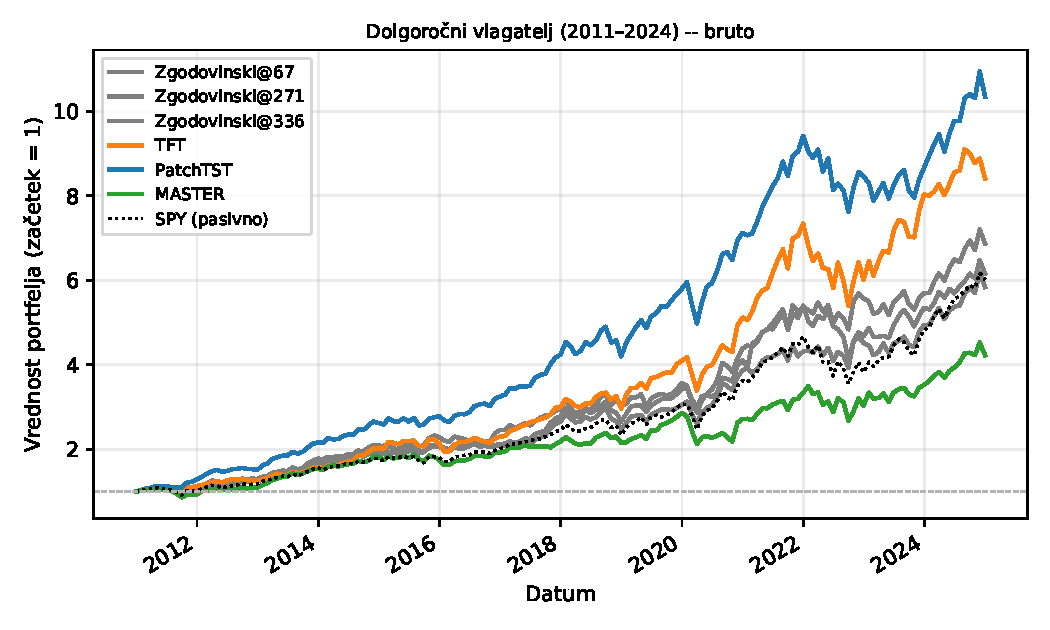
\includegraphics[height=\figheight]{fig/equity_all_longterm.pdf}\\[6pt]
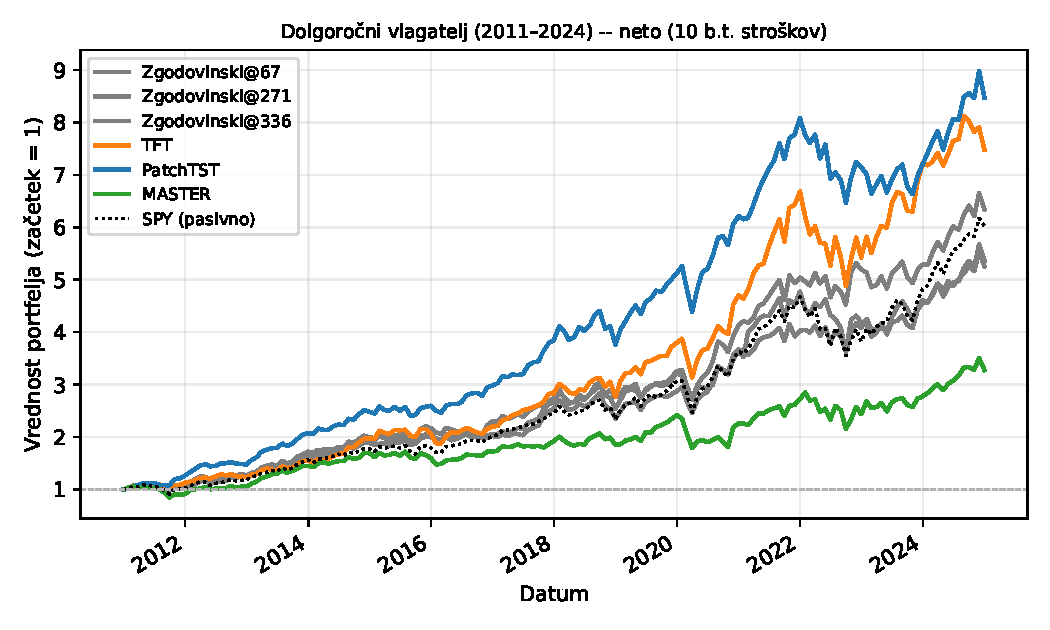
\includegraphics[height=\figheight]{fig/equity_all_longterm_net.pdf}
\caption{Gibanje vrednosti portfelja v dolgoročnem scenariju (2011--2024, $P{=}0{,}5$): bruto (zgoraj) in neto pri 10 b.t.\ (spodaj). Prisoten je survivorship bias.}
\label{fig:longterm}
\end{figure}

% ------------------------------------------------------------
% STABILITY AND TURNOVER
% ------------------------------------------------------------

\subsection{Stabilnost napovedi in promet portfelja}\label{sec:whytft}

Rezultati prejšnjih eksperimentov kažejo, da sama presečna napovedna korelacija še ne pojasni v celoti končne portfeljske uspešnosti. Zato v Tabeli~\ref{tab:whytft} kot dopolnilno analizo primerjamo letni promet portfelja; te mere ne obravnavamo kot glavno benchmark merilo.

\begin{table}[htbp]
\centering
\small
\caption{Letni promet portfelja za transformerske modele pri optimizatorju RD.}
\label{tab:whytft}
\begin{tabular}{lrrr}
\hline
Nabor & TFT & MASTER & PatchTST \\
\hline
Leow: razpršeni ETF  &  2,6 & 13,5 & 14,4 \\
Wang: S\&P~500       &  0,5 & 23,3 & 16,1 \\
Dolgoročni vlagatelj & 10,2 & 17,8 & 13,1 \\
\hline
Povprečje             &  4,4 & 18,2 & 14,5 \\
\hline
\end{tabular}
\end{table}

TFT v povprečju doseže letni promet $4{,}4$, MASTER $18{,}2$ in PatchTST $14{,}5$. Razlika med TFT in MASTER je posebej izrazita pri Wang S\&P~500 ($0{,}5$ proti $23{,}3$), kar neposredno pojasni razliko v neto Sharpovem količniku med modeloma.

Nižji promet je praktično pomemben, ker pomeni manj izrazite spremembe izbora in uteži med zaporednimi odločitvenimi trenutki ter praviloma manj trgovanja. Rezultate zato interpretiramo na ravni celotnega cevovoda: poleg napovedne kakovosti so pomembni tudi velikost napovedanih donosov, odziv optimizatorja na spremembe $\hat{\vec{\mu}}$ in posledična stabilnost portfeljskih odločitev.

% SKLEP
% ============================================================
\section{Sklep}\label{sec:sklep}

V magistrskem delu smo zasnovali cevovod za sestavo kardinalno omejenega portfelja, ki napovedovanje pričakovanih donosov in optimizacijo uteži obravnava kot dva ločena, vendar zaporedno povezana problema. Pričakovane donose~$\hat{\vec{\mu}}$ ocenjujemo s tremi arhitekturno različnimi transformerskimi modeli -- MASTER~\cite{li2024master}, TFT~\cite{lim2021tft} in PatchTST~\cite{nie2023patchtst}. Pri tem je nevronsko jedro vsakega modela čim tesneje povezano z uradno programsko izvedbo avtorjev, naše spremembe pa omejimo na podatkovni vmesnik, ameriški finančni nabor sredstev in pretvorbo izhoda v oceno pričakovanega donosa. Za vse tri napovedne modele uporabljamo isto vzorčno kovariančno matriko zgodovinskih donosov, zato primerjava izolira predvsem vpliv napovednega signala.

Iskanje uteži ob striktni kardinalni omejitvi rešujeta dve stohastični metahevristiki, rojenje delcev in simulirano ohlajanje. Obe rešujeta KONP in uporabljata isto ciljno funkcijo ter iste omejitve, razlikujeta pa se v strategiji preiskovanja prostora rešitev. Kakovost optimizacijskega dela preverjamo ločeno na standardnih problemih OR-Library, napovedni del pa na ločenem presečnem protokolu. Šele nato oba dela povežemo v postopno vrednotenje.

Pomemben metodološki vidik dela je sledljivost implementacij. PatchTST uporablja uradni \texttt{PatchTST\_backbone}, TFT odprtokodno knjižnico \texttt{pytorch-forecasting}~\cite{beitner2020pytorch}, MASTER pa izvorno arhitekturo avtorjev. Namestitvene skripte zabeležijo uporabljene revizije Git, zato je mogoče poleg nastavitev eksperimenta določiti tudi konkretno programsko različico posameznega modela. Pri metodah, ki jih zaradi drugačnega trga ali drugačne formulacije optimizacijskega problema ni mogoče dobesedno prenesti, prilagoditve eksplicitno opišemo.

Transformerski napovedni signal pozitivno vpliva na vrednost portfelja, a ne prek enega samega, dosledno najboljšega modela. TFT doseže najvišji Sharpov količnik v kriznem obdobju Leow All-Weather ($\LeowAWTFT$ proti $\LeowAWHistoricalTFT$ za ujemajočo osnovno linijo) in preseže svojo osnovno linijo tudi v dolgoročnem scenariju; PatchTST doseže najvišji absolutni Sharpe v dolgoročnem scenariju ($1{,}38$ proti $1{,}10$ za svojo osnovno linijo) in na naboru Aprea DJIA ($1{,}09$ proti $0{,}80$); MASTER pa je edini, ki jasno preseže svojo osnovno linijo na večjem naboru Aprea NASDAQ~100 ($1{,}23$ proti $1{,}03$), kjer TFT nasprotno izrazito zaostane ($0{,}55$ proti $0{,}94$). Pri Wangu sta TFT in PatchTST primerljiva ($\WangTFT$ oziroma $\WangPatchTST$) in se oba uvrstita med Wangov pristop \enquote{napovej, nato optimiziraj} in nevronski reševalnik CardNN-GS, ki komercialni reševalnik nadomesti z naučeno plastjo. Ključna ugotovitev, ki drži v vseh petih benchmarkih (Leow, Wang, Aprea DJIA, Aprea NASDAQ~100, dolgoročni scenarij), je, da v vsakem od njih \emph{vsaj en} transformer jasno preseže svojo ujemajočo zgodovinsko osnovno linijo -- kateri model to je, pa se sistematično menja z naborom sredstev in protokolom, kar kaže, da izbira napovednega modela ni univerzalna odločitev, temveč je odvisna od konteksta uporabe. Razlike med rojénjem delcev in simuliranim ohlajanjem so ob tem majhne in nekonsistentne prek scenarijev, kar kaže, da je kakovost napovednega signala~$\hat{\vec{\mu}}$ dominantni dejavnik portfeljske uspešnosti, ne izbira optimizatorja.

Delo ima več metodoloških omejitev. Zunanje študije uporabljajo različne nabore sredstev, časovna obdobja, ciljne funkcije in merila uspešnosti, zato njihove rezultate obravnavamo kot referenčne primerjave in ne kot popolne reprodukcije: pri Aprea in Sbaiz je razlika največja, saj njun $\Delta$CoVaR-kriterij ter omejitvi prometa in ESG niso implementirani, kardinalno omejitev $K{=}10$ pa dodamo mi, medtem ko pri njiju število pozicij ni omejeno, ampak je posledica intervalne meje uteži ($\lfloor 1/u_i \rfloor$). Nekateri javno rekonstruirani nabori vsebujejo pristranost zaradi preživetja, pri MASTER pa moramo kitajske tržne indekse nadomestiti z ameriškimi približki. Pri TFT in PatchTST se napovedno obdobje prilagaja posameznemu portfeljskemu protokolu, kar je potrebno za skupni cevovod, vendar pomeni odstopanje od posamezne referenčne eksperimentalne nastavitve. Rezultati Leow so poleg tega izrazito občutljivi na podrobnosti zgodnjega ustavljanja učenja (razdelek~\ref{sec:leow}), kar zahteva previdnost pri posploševanju iz katerekoli posamezne ponovitve tega protokola.

V prihodnje bi lahko cevovod razširili z natančnejšim modeliranjem transakcijskih stroškov in davkov, z robustnejšimi ocenami kovariančne matrike, s samodejnim izborom napovednega modela glede na tržni režim ter z merami repnega tveganja. Druga smer je tesnejša sklopitev napovedovanja in optimizacije v enoten pristop, naučen skozi optimizacijo~\cite{wang2023oneshot}.

% PATCHTST: v bib/bibliography.bib dodaj zapis iz patchtst_reference.bib.

% ============================================================
% BIBLIOGRAPHY
% ============================================================

% The acknowledgements content (not mandatory).
%\acknow{Zahvala.}

\bibliography{{bib/bibliography}}


\end{document}
